% Options for packages loaded elsewhere
\PassOptionsToPackage{unicode}{hyperref}
\PassOptionsToPackage{hyphens}{url}
%
\documentclass[
]{article}
\usepackage{lmodern}
\usepackage{amsmath}
\usepackage{ifxetex,ifluatex}
\ifnum 0\ifxetex 1\fi\ifluatex 1\fi=0 % if pdftex
  \usepackage[T1]{fontenc}
  \usepackage[utf8]{inputenc}
  \usepackage{textcomp} % provide euro and other symbols
  \usepackage{amssymb}
\else % if luatex or xetex
  \usepackage{unicode-math}
  \defaultfontfeatures{Scale=MatchLowercase}
  \defaultfontfeatures[\rmfamily]{Ligatures=TeX,Scale=1}
\fi
% Use upquote if available, for straight quotes in verbatim environments
\IfFileExists{upquote.sty}{\usepackage{upquote}}{}
\IfFileExists{microtype.sty}{% use microtype if available
  \usepackage[]{microtype}
  \UseMicrotypeSet[protrusion]{basicmath} % disable protrusion for tt fonts
}{}
\makeatletter
\@ifundefined{KOMAClassName}{% if non-KOMA class
  \IfFileExists{parskip.sty}{%
    \usepackage{parskip}
  }{% else
    \setlength{\parindent}{0pt}
    \setlength{\parskip}{6pt plus 2pt minus 1pt}}
}{% if KOMA class
  \KOMAoptions{parskip=half}}
\makeatother
\usepackage{xcolor}
\IfFileExists{xurl.sty}{\usepackage{xurl}}{} % add URL line breaks if available
\IfFileExists{bookmark.sty}{\usepackage{bookmark}}{\usepackage{hyperref}}
\hypersetup{
  pdftitle={descriptive},
  hidelinks,
  pdfcreator={LaTeX via pandoc}}
\urlstyle{same} % disable monospaced font for URLs
\usepackage[margin=1in]{geometry}
\usepackage{color}
\usepackage{fancyvrb}
\newcommand{\VerbBar}{|}
\newcommand{\VERB}{\Verb[commandchars=\\\{\}]}
\DefineVerbatimEnvironment{Highlighting}{Verbatim}{commandchars=\\\{\}}
% Add ',fontsize=\small' for more characters per line
\usepackage{framed}
\definecolor{shadecolor}{RGB}{248,248,248}
\newenvironment{Shaded}{\begin{snugshade}}{\end{snugshade}}
\newcommand{\AlertTok}[1]{\textcolor[rgb]{0.94,0.16,0.16}{#1}}
\newcommand{\AnnotationTok}[1]{\textcolor[rgb]{0.56,0.35,0.01}{\textbf{\textit{#1}}}}
\newcommand{\AttributeTok}[1]{\textcolor[rgb]{0.77,0.63,0.00}{#1}}
\newcommand{\BaseNTok}[1]{\textcolor[rgb]{0.00,0.00,0.81}{#1}}
\newcommand{\BuiltInTok}[1]{#1}
\newcommand{\CharTok}[1]{\textcolor[rgb]{0.31,0.60,0.02}{#1}}
\newcommand{\CommentTok}[1]{\textcolor[rgb]{0.56,0.35,0.01}{\textit{#1}}}
\newcommand{\CommentVarTok}[1]{\textcolor[rgb]{0.56,0.35,0.01}{\textbf{\textit{#1}}}}
\newcommand{\ConstantTok}[1]{\textcolor[rgb]{0.00,0.00,0.00}{#1}}
\newcommand{\ControlFlowTok}[1]{\textcolor[rgb]{0.13,0.29,0.53}{\textbf{#1}}}
\newcommand{\DataTypeTok}[1]{\textcolor[rgb]{0.13,0.29,0.53}{#1}}
\newcommand{\DecValTok}[1]{\textcolor[rgb]{0.00,0.00,0.81}{#1}}
\newcommand{\DocumentationTok}[1]{\textcolor[rgb]{0.56,0.35,0.01}{\textbf{\textit{#1}}}}
\newcommand{\ErrorTok}[1]{\textcolor[rgb]{0.64,0.00,0.00}{\textbf{#1}}}
\newcommand{\ExtensionTok}[1]{#1}
\newcommand{\FloatTok}[1]{\textcolor[rgb]{0.00,0.00,0.81}{#1}}
\newcommand{\FunctionTok}[1]{\textcolor[rgb]{0.00,0.00,0.00}{#1}}
\newcommand{\ImportTok}[1]{#1}
\newcommand{\InformationTok}[1]{\textcolor[rgb]{0.56,0.35,0.01}{\textbf{\textit{#1}}}}
\newcommand{\KeywordTok}[1]{\textcolor[rgb]{0.13,0.29,0.53}{\textbf{#1}}}
\newcommand{\NormalTok}[1]{#1}
\newcommand{\OperatorTok}[1]{\textcolor[rgb]{0.81,0.36,0.00}{\textbf{#1}}}
\newcommand{\OtherTok}[1]{\textcolor[rgb]{0.56,0.35,0.01}{#1}}
\newcommand{\PreprocessorTok}[1]{\textcolor[rgb]{0.56,0.35,0.01}{\textit{#1}}}
\newcommand{\RegionMarkerTok}[1]{#1}
\newcommand{\SpecialCharTok}[1]{\textcolor[rgb]{0.00,0.00,0.00}{#1}}
\newcommand{\SpecialStringTok}[1]{\textcolor[rgb]{0.31,0.60,0.02}{#1}}
\newcommand{\StringTok}[1]{\textcolor[rgb]{0.31,0.60,0.02}{#1}}
\newcommand{\VariableTok}[1]{\textcolor[rgb]{0.00,0.00,0.00}{#1}}
\newcommand{\VerbatimStringTok}[1]{\textcolor[rgb]{0.31,0.60,0.02}{#1}}
\newcommand{\WarningTok}[1]{\textcolor[rgb]{0.56,0.35,0.01}{\textbf{\textit{#1}}}}
\usepackage{longtable,booktabs}
\usepackage{calc} % for calculating minipage widths
% Correct order of tables after \paragraph or \subparagraph
\usepackage{etoolbox}
\makeatletter
\patchcmd\longtable{\par}{\if@noskipsec\mbox{}\fi\par}{}{}
\makeatother
% Allow footnotes in longtable head/foot
\IfFileExists{footnotehyper.sty}{\usepackage{footnotehyper}}{\usepackage{footnote}}
\makesavenoteenv{longtable}
\usepackage{graphicx}
\makeatletter
\def\maxwidth{\ifdim\Gin@nat@width>\linewidth\linewidth\else\Gin@nat@width\fi}
\def\maxheight{\ifdim\Gin@nat@height>\textheight\textheight\else\Gin@nat@height\fi}
\makeatother
% Scale images if necessary, so that they will not overflow the page
% margins by default, and it is still possible to overwrite the defaults
% using explicit options in \includegraphics[width, height, ...]{}
\setkeys{Gin}{width=\maxwidth,height=\maxheight,keepaspectratio}
% Set default figure placement to htbp
\makeatletter
\def\fps@figure{htbp}
\makeatother
\setlength{\emergencystretch}{3em} % prevent overfull lines
\providecommand{\tightlist}{%
  \setlength{\itemsep}{0pt}\setlength{\parskip}{0pt}}
\setcounter{secnumdepth}{-\maxdimen} % remove section numbering
\ifluatex
  \usepackage{selnolig}  % disable illegal ligatures
\fi

\title{descriptive}
\author{}
\date{\vspace{-2.5em}}

\begin{document}
\maketitle

\begin{Shaded}
\begin{Highlighting}[]
\NormalTok{daily\_indices }\OtherTok{\textless{}{-}} \FunctionTok{read\_rds}\NormalTok{(}\AttributeTok{file =} \StringTok{"data/daily\_indices.rds"}\NormalTok{)}


\CommentTok{\# daily\_indices \textless{}{-} read\_rds(file = "E:/data/daily\_indices.rds") \%\textgreater{}\% }
\CommentTok{\#   rename(date = \textasciigrave{}lubridate::date(local\_dttm)\textasciigrave{}) \%\textgreater{}\% }
\CommentTok{\#   mutate(wbgt\_f\_mean = weathermetrics::celsius.to.fahrenheit(wbgt\_u\_mean),}
\CommentTok{\#          installation = recode(installation, }
\CommentTok{\#                 \textasciigrave{}pensacola\_nas\textasciigrave{} = "pensacola",}
\CommentTok{\#                 \textasciigrave{}portsmouth\_nmc\textasciigrave{} = "portsmouth"))}

\CommentTok{\# write\_rds(daily\_indices, file = "data/daily\_indices.rds")}


\NormalTok{cc\_exposure\_df }\OtherTok{\textless{}{-}}
  \FunctionTok{read\_rds}\NormalTok{(}\AttributeTok{file =} \StringTok{"data/cc\_exposure\_df.rds"}\NormalTok{)}

\CommentTok{\# cc\_exposure\_df \textless{}{-}}
\CommentTok{\#   read\_rds(file = "E:/data/cc\_exposure\_df.rds") \%\textgreater{}\% }
\CommentTok{\#   mutate(wbgt\_f\_mean = weathermetrics::celsius.to.fahrenheit(wbgt\_u\_mean))}


\NormalTok{cc\_exposure\_df }\SpecialCharTok{\%\textgreater{}\%} 
  \FunctionTok{count}\NormalTok{(installation\_name) }\SpecialCharTok{\%\textgreater{}\%} \FunctionTok{View}\NormalTok{() }\CommentTok{\#24 installations}


\CommentTok{\# cc\_exposure\_df \textless{}{-}}
\CommentTok{\#   cc\_exposure\_df \%\textgreater{}\% }
\CommentTok{\#      mutate(installation\_name = as\_factor(installation\_name),}
\CommentTok{\#        installation\_name = recode(installation\_name,}
\CommentTok{\#         "mcb\_camp\_lejeune" = "camp\_lejeune",}
\CommentTok{\#         "mcb\_camp\_pendleton" = "camp\_pendleton",}
\CommentTok{\#         "fort\_benning\_ga" = "fort\_benning",}
\CommentTok{\#         "fort\_sam\_houston" = "jbsa",}
\CommentTok{\#         "mcrd\_beaufort\_parris\_island" = "parris\_island",}
\CommentTok{\#         "mcb\_quantico" = "quantico",}
\CommentTok{\#         "twentynine\_palms\_main\_base" = "twentynine\_palms")) }


\CommentTok{\# write\_rds(cc\_exposure\_df, file = "data/cc\_exposure\_df.rds")}
\CommentTok{\# write\_rds(daily\_indices, file = "data/daily\_indices.rds")}
\end{Highlighting}
\end{Shaded}

\hypertarget{counts-by-service---installation}{%
\subsubsection{Counts by service -
installation}\label{counts-by-service---installation}}

\begin{Shaded}
\begin{Highlighting}[]
\NormalTok{base\_service\_counts }\OtherTok{\textless{}{-}}
\NormalTok{  cc\_exposure\_df }\SpecialCharTok{\%\textgreater{}\%} 
    \FunctionTok{count}\NormalTok{(installation\_name, service) }\SpecialCharTok{\%\textgreater{}\%} 
    \FunctionTok{spread}\NormalTok{(service, n, }\AttributeTok{fill =} \DecValTok{0}\NormalTok{) }


\CommentTok{\# rank case occurrence by service for each installation; filter top}

\NormalTok{base\_service\_rank }\OtherTok{\textless{}{-}}
\NormalTok{  cc\_exposure\_df }\SpecialCharTok{\%\textgreater{}\%} 
    \FunctionTok{count}\NormalTok{(installation\_name, service) }\SpecialCharTok{\%\textgreater{}\%} 
    \FunctionTok{group\_by}\NormalTok{(installation\_name) }\SpecialCharTok{\%\textgreater{}\%} 
    \FunctionTok{mutate}\NormalTok{(}\AttributeTok{rank =} \FunctionTok{rank}\NormalTok{(}\SpecialCharTok{{-}}\NormalTok{n)) }\SpecialCharTok{\%\textgreater{}\%} 
    \FunctionTok{filter}\NormalTok{(rank }\SpecialCharTok{==} \DecValTok{1}\NormalTok{)}

\NormalTok{base\_service\_df }\OtherTok{\textless{}{-}}
\NormalTok{  base\_service\_counts }\SpecialCharTok{\%\textgreater{}\%} 
    \FunctionTok{right\_join}\NormalTok{(base\_service\_rank }\SpecialCharTok{\%\textgreater{}\%} 
\NormalTok{                 dplyr}\SpecialCharTok{::}\FunctionTok{select}\NormalTok{(installation\_name, service), }\AttributeTok{by =} \StringTok{"installation\_name"}\NormalTok{) }


\NormalTok{base\_service\_df }\SpecialCharTok{\%\textgreater{}\%} 
  \FunctionTok{count}\NormalTok{(service)}
\end{Highlighting}
\end{Shaded}

\begin{verbatim}
## # A tibble: 4 x 2
##   service     n
##   <chr>   <int>
## 1 A          14
## 2 F           2
## 3 M           6
## 4 N           2
\end{verbatim}

\hypertarget{geographic-climate-region}{%
\subsubsection{Geographic / climate
region}\label{geographic-climate-region}}

\url{https://www.ncdc.noaa.gov/monitoring-references/maps/us-climate-regions.php}

Through climate analysis, National Centers for Environmental Information
scientists have identified nine climatically consistent regions within
the contiguous United States which are useful for putting current
climate anomalies into a historical perspective (Karl and Koss, 1984).

\begin{Shaded}
\begin{Highlighting}[]
\NormalTok{base\_service\_df}\SpecialCharTok{$}\NormalTok{installation\_name}
\end{Highlighting}
\end{Shaded}

\begin{verbatim}
##  [1] fort_benning       fort_bragg         camp_lejeune       parris_island     
##  [5] fort_campbell      fort_polk          fort_jackson       camp_pendleton    
##  [9] fort_hood          mcrd_san_diego     fort_stewart       jbsa              
## [13] quantico           twentynine_palms   fort_sill          fort_leonard_wood 
## [17] fort_riley         ntc_and_fort_irwin fort_knox          fort_bliss        
## [21] portsmouth         pensacola          fort_gordon        eglin_afb         
## 24 Levels: fort_benning fort_bragg camp_lejeune parris_island ... eglin_afb
\end{verbatim}

\begin{Shaded}
\begin{Highlighting}[]
\CommentTok{\# Assign U.S. Climate regions}

\DocumentationTok{\#\# 1st column}
\NormalTok{installation\_name }\OtherTok{\textless{}{-}}\NormalTok{ base\_service\_df}\SpecialCharTok{$}\NormalTok{installation\_name }
\DocumentationTok{\#\# 2nd column}
\NormalTok{region }\OtherTok{\textless{}{-}} \FunctionTok{c}\NormalTok{(}\StringTok{"Southeast"}\NormalTok{, }\StringTok{"Southeast"}\NormalTok{, }\StringTok{"Southeast"}\NormalTok{, }\StringTok{"Southeast"}\NormalTok{, }\StringTok{"Ohio Valley"}\NormalTok{, }\StringTok{"South"}\NormalTok{, }
            \StringTok{"Southeast"}\NormalTok{, }\StringTok{"West"}\NormalTok{, }\StringTok{"South"}\NormalTok{, }\StringTok{"West"}\NormalTok{, }\StringTok{"Southeast"}\NormalTok{, }\StringTok{"South"}\NormalTok{,}
            \StringTok{"Southeast"}\NormalTok{, }\StringTok{"West"}\NormalTok{, }\StringTok{"South"}\NormalTok{, }\StringTok{"Ohio Valley"}\NormalTok{, }\StringTok{"South"}\NormalTok{, }\StringTok{"West"}\NormalTok{,}
            \StringTok{"Ohio Valley"}\NormalTok{, }\StringTok{"South"}\NormalTok{, }\StringTok{"Southeast"}\NormalTok{, }\StringTok{"Southeast"}\NormalTok{, }\StringTok{"Southeast"}\NormalTok{, }\StringTok{"Southeast"}
\NormalTok{            )}

\NormalTok{climate\_regions }\OtherTok{\textless{}{-}} \FunctionTok{data.frame}\NormalTok{(installation\_name, region) }\SpecialCharTok{\%\textgreater{}\%} 
  \FunctionTok{as\_tibble}\NormalTok{()}
  

\NormalTok{base\_service\_df }\OtherTok{\textless{}{-}} 
\NormalTok{  base\_service\_df }\SpecialCharTok{\%\textgreater{}\%} 
    \FunctionTok{right\_join}\NormalTok{(climate\_regions, }\AttributeTok{by =} \StringTok{"installation\_name"}\NormalTok{) }


\NormalTok{base\_service\_df }\OtherTok{\textless{}{-}}
\NormalTok{  base\_service\_df }\SpecialCharTok{\%\textgreater{}\%} 
    \FunctionTok{mutate}\NormalTok{(}\AttributeTok{service =} \FunctionTok{recode}\NormalTok{(service,}
          \StringTok{"A"} \OtherTok{=} \StringTok{"Army"}\NormalTok{,}
          \StringTok{"C"} \OtherTok{=} \StringTok{"Coast Guard"}\NormalTok{,}
          \StringTok{"F"} \OtherTok{=} \StringTok{"Air Force"}\NormalTok{,}
          \StringTok{"M"} \OtherTok{=} \StringTok{"Marine Corps"}\NormalTok{,}
          \StringTok{"N"} \OtherTok{=} \StringTok{"Navy"}\NormalTok{))}


\CommentTok{\#write\_rds(base\_service\_df, file = "data/base\_service\_df.rds")}
  


\NormalTok{base\_service\_df }\SpecialCharTok{\%\textgreater{}\%} 
  \FunctionTok{ggplot}\NormalTok{(}\FunctionTok{aes}\NormalTok{(region)) }\SpecialCharTok{+}
    \FunctionTok{geom\_bar}\NormalTok{() }\SpecialCharTok{+}
    \FunctionTok{theme\_bw}\NormalTok{()}
\end{Highlighting}
\end{Shaded}

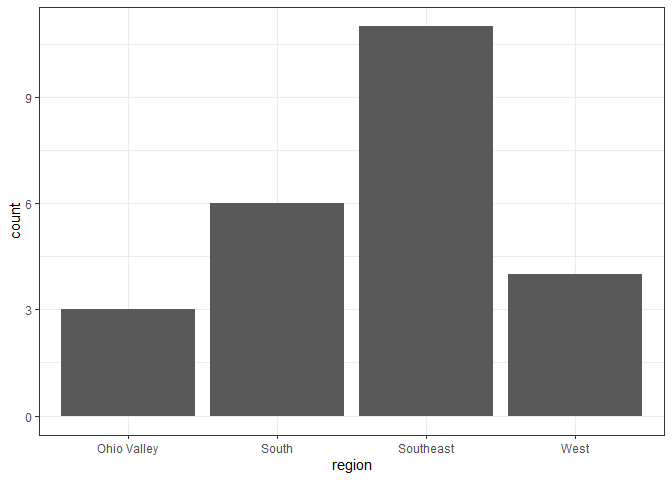
\includegraphics{descriptive_files/figure-latex/unnamed-chunk-3-1.pdf}

\begin{Shaded}
\begin{Highlighting}[]
\NormalTok{base\_service\_df }\SpecialCharTok{\%\textgreater{}\%} 
  \FunctionTok{ggplot}\NormalTok{(}\FunctionTok{aes}\NormalTok{(region, }\AttributeTok{fill =}\NormalTok{ service)) }\SpecialCharTok{+}
    \FunctionTok{geom\_bar}\NormalTok{(}\AttributeTok{position =} \FunctionTok{position\_dodge}\NormalTok{()) }\SpecialCharTok{+}
    \FunctionTok{theme\_bw}\NormalTok{()}
\end{Highlighting}
\end{Shaded}

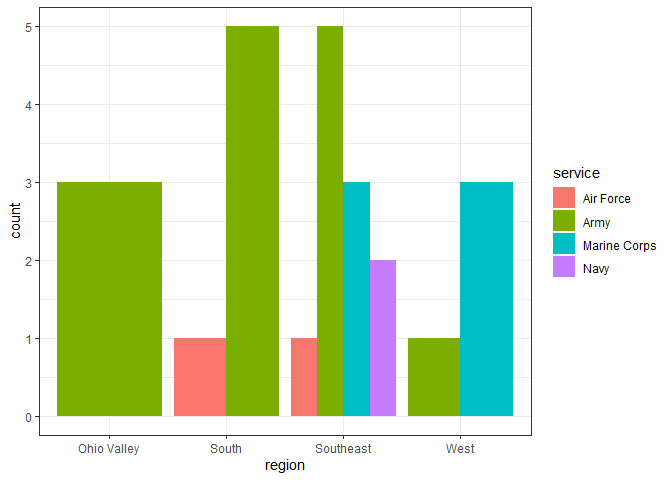
\includegraphics{descriptive_files/figure-latex/unnamed-chunk-3-2.pdf}

\begin{Shaded}
\begin{Highlighting}[]
\CommentTok{\# Cross{-}tab service and region}
\NormalTok{base\_service\_df }\SpecialCharTok{\%\textgreater{}\%} 
  \FunctionTok{group\_by}\NormalTok{(service, region) }\SpecialCharTok{\%\textgreater{}\%} 
  \FunctionTok{summarise}\NormalTok{(}\AttributeTok{n =} \FunctionTok{n}\NormalTok{()) }\SpecialCharTok{\%\textgreater{}\%} 
  \FunctionTok{spread}\NormalTok{(region, n)}
\end{Highlighting}
\end{Shaded}

\begin{verbatim}
## `summarise()` regrouping output by 'service' (override with `.groups` argument)
\end{verbatim}

\begin{verbatim}
## # A tibble: 4 x 5
## # Groups:   service [4]
##   service      `Ohio Valley` South Southeast  West
##   <chr>                <int> <int>     <int> <int>
## 1 Air Force               NA     1         1    NA
## 2 Army                     3     5         5     1
## 3 Marine Corps            NA    NA         3     3
## 4 Navy                    NA    NA         2    NA
\end{verbatim}

\begin{Shaded}
\begin{Highlighting}[]
\NormalTok{base\_service\_df }\SpecialCharTok{\%\textgreater{}\%} 
  \FunctionTok{group\_by}\NormalTok{(service, region) }\SpecialCharTok{\%\textgreater{}\%} 
  \FunctionTok{summarise}\NormalTok{(}\AttributeTok{n =} \FunctionTok{n}\NormalTok{()) }\SpecialCharTok{\%\textgreater{}\%} 
  \FunctionTok{spread}\NormalTok{(region, n) }\SpecialCharTok{\%\textgreater{}\%} 
\NormalTok{  knitr}\SpecialCharTok{::}\FunctionTok{kable}\NormalTok{()}
\end{Highlighting}
\end{Shaded}

\begin{verbatim}
## `summarise()` regrouping output by 'service' (override with `.groups` argument)
\end{verbatim}

\begin{longtable}[]{@{}lrrrr@{}}
\toprule
service & Ohio Valley & South & Southeast & West\tabularnewline
\midrule
\endhead
Air Force & NA & 1 & 1 & NA\tabularnewline
Army & 3 & 5 & 5 & 1\tabularnewline
Marine Corps & NA & NA & 3 & 3\tabularnewline
Navy & NA & NA & 2 & NA\tabularnewline
\bottomrule
\end{longtable}

\hypertarget{outcome-table}{%
\subsection{Outcome table}\label{outcome-table}}

\begin{Shaded}
\begin{Highlighting}[]
\NormalTok{to\_table1 }\OtherTok{\textless{}{-}}
\NormalTok{  cc\_exposure\_df }\SpecialCharTok{\%\textgreater{}\%} 
    \FunctionTok{filter}\NormalTok{(case }\SpecialCharTok{==} \DecValTok{1}\NormalTok{) }\SpecialCharTok{\%\textgreater{}\%} 
\NormalTok{    dplyr}\SpecialCharTok{::}\FunctionTok{select}\NormalTok{(installation\_name, source, age, sex, race\_ethnic, service, grade, hsi) }\SpecialCharTok{\%\textgreater{}\%} 
       \FunctionTok{mutate}\NormalTok{(}\AttributeTok{service =} \FunctionTok{recode}\NormalTok{(service,}
            \StringTok{"A"} \OtherTok{=} \StringTok{"Army"}\NormalTok{,}
            \StringTok{"C"} \OtherTok{=} \StringTok{"Coast Guard"}\NormalTok{,}
            \StringTok{"F"} \OtherTok{=} \StringTok{"Air Force"}\NormalTok{,}
            \StringTok{"M"} \OtherTok{=} \StringTok{"Marine Corps"}\NormalTok{,}
            \StringTok{"N"} \OtherTok{=} \StringTok{"Navy"}\NormalTok{),}
            \AttributeTok{source =} \FunctionTok{recode}\NormalTok{(source,}
            \StringTok{"INPATIENT"} \OtherTok{=} \StringTok{"In{-}Patient"}\NormalTok{,}
            \StringTok{"OUTPATIENT"} \OtherTok{=} \StringTok{"Out{-}Patient"}\NormalTok{,}
            \StringTok{"RME"} \OtherTok{=} \StringTok{"Reportable Event"}\NormalTok{),}
            \AttributeTok{hsi =} \FunctionTok{recode}\NormalTok{(hsi,}
            \StringTok{"heat\_exhaustion"} \OtherTok{=} \StringTok{"Heat Exhaustion"}\NormalTok{,}
            \StringTok{"heat\_stroke"} \OtherTok{=} \StringTok{"Heat Stroke"}\NormalTok{),}
            \AttributeTok{sex =} \FunctionTok{recode}\NormalTok{(sex,}
            \StringTok{"F"} \OtherTok{=} \StringTok{"Female"}\NormalTok{,}
            \StringTok{"M"} \OtherTok{=} \StringTok{"Male"}\NormalTok{,}
            \StringTok{"Z"} \OtherTok{=} \StringTok{"Unknown"}\NormalTok{)}
\NormalTok{            ) }\SpecialCharTok{\%\textgreater{}\%} 
  \FunctionTok{left\_join}\NormalTok{(climate\_regions, }\AttributeTok{by =} \StringTok{"installation\_name"}\NormalTok{) }\SpecialCharTok{\%\textgreater{}\%} 
  \FunctionTok{mutate\_if}\NormalTok{(is.character, as.factor) }\SpecialCharTok{\%\textgreater{}\%} 
            \FunctionTok{mutate}\NormalTok{(}\AttributeTok{age =} \FunctionTok{fct\_relevel}\NormalTok{(age, }\StringTok{"\textgreater{}=40"}\NormalTok{, }\AttributeTok{after =} \ConstantTok{Inf}\NormalTok{))}


\FunctionTok{label}\NormalTok{(to\_table1}\SpecialCharTok{$}\NormalTok{hsi) }\OtherTok{\textless{}{-}} \StringTok{"HSI Diagnosis"}
\FunctionTok{label}\NormalTok{(to\_table1}\SpecialCharTok{$}\NormalTok{age) }\OtherTok{\textless{}{-}} \StringTok{"Age Group"}
\FunctionTok{label}\NormalTok{(to\_table1}\SpecialCharTok{$}\NormalTok{sex) }\OtherTok{\textless{}{-}} \StringTok{"Sex"}
\FunctionTok{label}\NormalTok{(to\_table1}\SpecialCharTok{$}\NormalTok{race\_ethnic) }\OtherTok{\textless{}{-}} \StringTok{"Race/Ethnicity"}
\FunctionTok{label}\NormalTok{(to\_table1}\SpecialCharTok{$}\NormalTok{grade) }\OtherTok{\textless{}{-}} \StringTok{"Grade Group"}
\FunctionTok{label}\NormalTok{(to\_table1}\SpecialCharTok{$}\NormalTok{service) }\OtherTok{\textless{}{-}} \StringTok{"Service Branch"}
\FunctionTok{label}\NormalTok{(to\_table1}\SpecialCharTok{$}\NormalTok{region) }\OtherTok{\textless{}{-}} \StringTok{"NOAA NCEI Climate Region"}


\NormalTok{table1}\SpecialCharTok{::}\FunctionTok{table1}\NormalTok{(}\SpecialCharTok{\textasciitilde{}}\NormalTok{ hsi }\SpecialCharTok{+}\NormalTok{ sex }\SpecialCharTok{+}\NormalTok{ age }\SpecialCharTok{+}\NormalTok{ sex }\SpecialCharTok{+}\NormalTok{ grade }\SpecialCharTok{+}\NormalTok{ race\_ethnic  }\SpecialCharTok{|}\NormalTok{ source, }\AttributeTok{data =}\NormalTok{ to\_table1)}
\end{Highlighting}
\end{Shaded}

\begin{verbatim}
## [1] "<table class=\"Rtable1\">\n<thead>\n<tr>\n<th class='rowlabel firstrow lastrow'></th>\n<th class='firstrow lastrow'><span class='stratlabel'>In-Patient<br><span class='stratn'>(N=3274)</span></span></th>\n<th class='firstrow lastrow'><span class='stratlabel'>Out-Patient<br><span class='stratn'>(N=17856)</span></span></th>\n<th class='firstrow lastrow'><span class='stratlabel'>Reportable Event<br><span class='stratn'>(N=10512)</span></span></th>\n<th class='firstrow lastrow'><span class='stratlabel'>Overall<br><span class='stratn'>(N=31642)</span></span></th>\n</tr>\n</thead>\n<tbody>\n<tr>\n<td class='rowlabel firstrow'><span class='varlabel'>HSI Diagnosis</span></td>\n<td class='firstrow'></td>\n<td class='firstrow'></td>\n<td class='firstrow'></td>\n<td class='firstrow'></td>\n</tr>\n<tr>\n<td class='rowlabel'>Heat Exhaustion</td>\n<td>1328 (40.6%)</td>\n<td>14902 (83.5%)</td>\n<td>8983 (85.5%)</td>\n<td>25213 (79.7%)</td>\n</tr>\n<tr>\n<td class='rowlabel lastrow'>Heat Stroke</td>\n<td class='lastrow'>1946 (59.4%)</td>\n<td class='lastrow'>2954 (16.5%)</td>\n<td class='lastrow'>1529 (14.5%)</td>\n<td class='lastrow'>6429 (20.3%)</td>\n</tr>\n<tr>\n<td class='rowlabel firstrow'><span class='varlabel'>Sex</span></td>\n<td class='firstrow'></td>\n<td class='firstrow'></td>\n<td class='firstrow'></td>\n<td class='firstrow'></td>\n</tr>\n<tr>\n<td class='rowlabel'>Female</td>\n<td>207 (6.3%)</td>\n<td>2693 (15.1%)</td>\n<td>1852 (17.6%)</td>\n<td>4752 (15.0%)</td>\n</tr>\n<tr>\n<td class='rowlabel'>Male</td>\n<td>3066 (93.6%)</td>\n<td>15162 (84.9%)</td>\n<td>8660 (82.4%)</td>\n<td>26888 (85.0%)</td>\n</tr>\n<tr>\n<td class='rowlabel lastrow'>Unknown</td>\n<td class='lastrow'>1 (0.0%)</td>\n<td class='lastrow'>1 (0.0%)</td>\n<td class='lastrow'>0 (0%)</td>\n<td class='lastrow'>2 (0.0%)</td>\n</tr>\n<tr>\n<td class='rowlabel firstrow'><span class='varlabel'>Age Group</span></td>\n<td class='firstrow'></td>\n<td class='firstrow'></td>\n<td class='firstrow'></td>\n<td class='firstrow'></td>\n</tr>\n<tr>\n<td class='rowlabel'><20</td>\n<td>683 (20.9%)</td>\n<td>4488 (25.1%)</td>\n<td>2848 (27.1%)</td>\n<td>8019 (25.3%)</td>\n</tr>\n<tr>\n<td class='rowlabel'>20-24</td>\n<td>1377 (42.1%)</td>\n<td>7699 (43.1%)</td>\n<td>4652 (44.3%)</td>\n<td>13728 (43.4%)</td>\n</tr>\n<tr>\n<td class='rowlabel'>25-29</td>\n<td>657 (20.1%)</td>\n<td>3182 (17.8%)</td>\n<td>1779 (16.9%)</td>\n<td>5618 (17.8%)</td>\n</tr>\n<tr>\n<td class='rowlabel'>30-34</td>\n<td>340 (10.4%)</td>\n<td>1381 (7.7%)</td>\n<td>737 (7.0%)</td>\n<td>2458 (7.8%)</td>\n</tr>\n<tr>\n<td class='rowlabel'>35-39</td>\n<td>141 (4.3%)</td>\n<td>686 (3.8%)</td>\n<td>334 (3.2%)</td>\n<td>1161 (3.7%)</td>\n</tr>\n<tr>\n<td class='rowlabel'>>=40</td>\n<td>75 (2.3%)</td>\n<td>417 (2.3%)</td>\n<td>158 (1.5%)</td>\n<td>650 (2.1%)</td>\n</tr>\n<tr>\n<td class='rowlabel lastrow'>Missing</td>\n<td class='lastrow'>1 (0.0%)</td>\n<td class='lastrow'>3 (0.0%)</td>\n<td class='lastrow'>4 (0.0%)</td>\n<td class='lastrow'>8 (0.0%)</td>\n</tr>\n<tr>\n<td class='rowlabel firstrow'><span class='varlabel'>Grade Group</span></td>\n<td class='firstrow'></td>\n<td class='firstrow'></td>\n<td class='firstrow'></td>\n<td class='firstrow'></td>\n</tr>\n<tr>\n<td class='rowlabel'>E1-E4</td>\n<td>2173 (66.4%)</td>\n<td>13183 (73.8%)</td>\n<td>8276 (78.7%)</td>\n<td>23632 (74.7%)</td>\n</tr>\n<tr>\n<td class='rowlabel'>E5-E9</td>\n<td>644 (19.7%)</td>\n<td>3122 (17.5%)</td>\n<td>1606 (15.3%)</td>\n<td>5372 (17.0%)</td>\n</tr>\n<tr>\n<td class='rowlabel'>O1-O3/W1-W3</td>\n<td>420 (12.8%)</td>\n<td>1413 (7.9%)</td>\n<td>580 (5.5%)</td>\n<td>2413 (7.6%)</td>\n</tr>\n<tr>\n<td class='rowlabel'>O4-O10/W4-W5</td>\n<td>37 (1.1%)</td>\n<td>137 (0.8%)</td>\n<td>50 (0.5%)</td>\n<td>224 (0.7%)</td>\n</tr>\n<tr>\n<td class='rowlabel lastrow'>Missing</td>\n<td class='lastrow'>0 (0%)</td>\n<td class='lastrow'>1 (0.0%)</td>\n<td class='lastrow'>0 (0%)</td>\n<td class='lastrow'>1 (0.0%)</td>\n</tr>\n<tr>\n<td class='rowlabel firstrow'><span class='varlabel'>Race/Ethnicity</span></td>\n<td class='firstrow'></td>\n<td class='firstrow'></td>\n<td class='firstrow'></td>\n<td class='firstrow'></td>\n</tr>\n<tr>\n<td class='rowlabel'>American Indian/Alaskan Native</td>\n<td>35 (1.1%)</td>\n<td>112 (0.6%)</td>\n<td>113 (1.1%)</td>\n<td>260 (0.8%)</td>\n</tr>\n<tr>\n<td class='rowlabel'>Asian/Pacific Islander</td>\n<td>162 (4.9%)</td>\n<td>756 (4.2%)</td>\n<td>519 (4.9%)</td>\n<td>1437 (4.5%)</td>\n</tr>\n<tr>\n<td class='rowlabel'>Hispanic</td>\n<td>363 (11.1%)</td>\n<td>2074 (11.6%)</td>\n<td>1221 (11.6%)</td>\n<td>3658 (11.6%)</td>\n</tr>\n<tr>\n<td class='rowlabel'>Non-Hispanic Black</td>\n<td>575 (17.6%)</td>\n<td>3076 (17.2%)</td>\n<td>2067 (19.7%)</td>\n<td>5718 (18.1%)</td>\n</tr>\n<tr>\n<td class='rowlabel'>Non-Hispanic White</td>\n<td>2044 (62.4%)</td>\n<td>11143 (62.4%)</td>\n<td>6303 (60.0%)</td>\n<td>19490 (61.6%)</td>\n</tr>\n<tr>\n<td class='rowlabel'>Other</td>\n<td>42 (1.3%)</td>\n<td>357 (2.0%)</td>\n<td>149 (1.4%)</td>\n<td>548 (1.7%)</td>\n</tr>\n<tr>\n<td class='rowlabel lastrow'>Unknown</td>\n<td class='lastrow'>53 (1.6%)</td>\n<td class='lastrow'>338 (1.9%)</td>\n<td class='lastrow'>140 (1.3%)</td>\n<td class='lastrow'>531 (1.7%)</td>\n</tr>\n</tbody>\n</table>\n"
\end{verbatim}

\begin{Shaded}
\begin{Highlighting}[]
\NormalTok{table1}\SpecialCharTok{::}\FunctionTok{table1}\NormalTok{(}\SpecialCharTok{\textasciitilde{}}\NormalTok{ hsi }\SpecialCharTok{+}\NormalTok{ sex }\SpecialCharTok{+}\NormalTok{ age }\SpecialCharTok{+}\NormalTok{ sex }\SpecialCharTok{+}\NormalTok{ grade   }\SpecialCharTok{|}\NormalTok{ source, }\AttributeTok{data =}\NormalTok{ to\_table1)  }
\end{Highlighting}
\end{Shaded}

\begin{verbatim}
## [1] "<table class=\"Rtable1\">\n<thead>\n<tr>\n<th class='rowlabel firstrow lastrow'></th>\n<th class='firstrow lastrow'><span class='stratlabel'>In-Patient<br><span class='stratn'>(N=3274)</span></span></th>\n<th class='firstrow lastrow'><span class='stratlabel'>Out-Patient<br><span class='stratn'>(N=17856)</span></span></th>\n<th class='firstrow lastrow'><span class='stratlabel'>Reportable Event<br><span class='stratn'>(N=10512)</span></span></th>\n<th class='firstrow lastrow'><span class='stratlabel'>Overall<br><span class='stratn'>(N=31642)</span></span></th>\n</tr>\n</thead>\n<tbody>\n<tr>\n<td class='rowlabel firstrow'><span class='varlabel'>HSI Diagnosis</span></td>\n<td class='firstrow'></td>\n<td class='firstrow'></td>\n<td class='firstrow'></td>\n<td class='firstrow'></td>\n</tr>\n<tr>\n<td class='rowlabel'>Heat Exhaustion</td>\n<td>1328 (40.6%)</td>\n<td>14902 (83.5%)</td>\n<td>8983 (85.5%)</td>\n<td>25213 (79.7%)</td>\n</tr>\n<tr>\n<td class='rowlabel lastrow'>Heat Stroke</td>\n<td class='lastrow'>1946 (59.4%)</td>\n<td class='lastrow'>2954 (16.5%)</td>\n<td class='lastrow'>1529 (14.5%)</td>\n<td class='lastrow'>6429 (20.3%)</td>\n</tr>\n<tr>\n<td class='rowlabel firstrow'><span class='varlabel'>Sex</span></td>\n<td class='firstrow'></td>\n<td class='firstrow'></td>\n<td class='firstrow'></td>\n<td class='firstrow'></td>\n</tr>\n<tr>\n<td class='rowlabel'>Female</td>\n<td>207 (6.3%)</td>\n<td>2693 (15.1%)</td>\n<td>1852 (17.6%)</td>\n<td>4752 (15.0%)</td>\n</tr>\n<tr>\n<td class='rowlabel'>Male</td>\n<td>3066 (93.6%)</td>\n<td>15162 (84.9%)</td>\n<td>8660 (82.4%)</td>\n<td>26888 (85.0%)</td>\n</tr>\n<tr>\n<td class='rowlabel lastrow'>Unknown</td>\n<td class='lastrow'>1 (0.0%)</td>\n<td class='lastrow'>1 (0.0%)</td>\n<td class='lastrow'>0 (0%)</td>\n<td class='lastrow'>2 (0.0%)</td>\n</tr>\n<tr>\n<td class='rowlabel firstrow'><span class='varlabel'>Age Group</span></td>\n<td class='firstrow'></td>\n<td class='firstrow'></td>\n<td class='firstrow'></td>\n<td class='firstrow'></td>\n</tr>\n<tr>\n<td class='rowlabel'><20</td>\n<td>683 (20.9%)</td>\n<td>4488 (25.1%)</td>\n<td>2848 (27.1%)</td>\n<td>8019 (25.3%)</td>\n</tr>\n<tr>\n<td class='rowlabel'>20-24</td>\n<td>1377 (42.1%)</td>\n<td>7699 (43.1%)</td>\n<td>4652 (44.3%)</td>\n<td>13728 (43.4%)</td>\n</tr>\n<tr>\n<td class='rowlabel'>25-29</td>\n<td>657 (20.1%)</td>\n<td>3182 (17.8%)</td>\n<td>1779 (16.9%)</td>\n<td>5618 (17.8%)</td>\n</tr>\n<tr>\n<td class='rowlabel'>30-34</td>\n<td>340 (10.4%)</td>\n<td>1381 (7.7%)</td>\n<td>737 (7.0%)</td>\n<td>2458 (7.8%)</td>\n</tr>\n<tr>\n<td class='rowlabel'>35-39</td>\n<td>141 (4.3%)</td>\n<td>686 (3.8%)</td>\n<td>334 (3.2%)</td>\n<td>1161 (3.7%)</td>\n</tr>\n<tr>\n<td class='rowlabel'>>=40</td>\n<td>75 (2.3%)</td>\n<td>417 (2.3%)</td>\n<td>158 (1.5%)</td>\n<td>650 (2.1%)</td>\n</tr>\n<tr>\n<td class='rowlabel lastrow'>Missing</td>\n<td class='lastrow'>1 (0.0%)</td>\n<td class='lastrow'>3 (0.0%)</td>\n<td class='lastrow'>4 (0.0%)</td>\n<td class='lastrow'>8 (0.0%)</td>\n</tr>\n<tr>\n<td class='rowlabel firstrow'><span class='varlabel'>Grade Group</span></td>\n<td class='firstrow'></td>\n<td class='firstrow'></td>\n<td class='firstrow'></td>\n<td class='firstrow'></td>\n</tr>\n<tr>\n<td class='rowlabel'>E1-E4</td>\n<td>2173 (66.4%)</td>\n<td>13183 (73.8%)</td>\n<td>8276 (78.7%)</td>\n<td>23632 (74.7%)</td>\n</tr>\n<tr>\n<td class='rowlabel'>E5-E9</td>\n<td>644 (19.7%)</td>\n<td>3122 (17.5%)</td>\n<td>1606 (15.3%)</td>\n<td>5372 (17.0%)</td>\n</tr>\n<tr>\n<td class='rowlabel'>O1-O3/W1-W3</td>\n<td>420 (12.8%)</td>\n<td>1413 (7.9%)</td>\n<td>580 (5.5%)</td>\n<td>2413 (7.6%)</td>\n</tr>\n<tr>\n<td class='rowlabel'>O4-O10/W4-W5</td>\n<td>37 (1.1%)</td>\n<td>137 (0.8%)</td>\n<td>50 (0.5%)</td>\n<td>224 (0.7%)</td>\n</tr>\n<tr>\n<td class='rowlabel lastrow'>Missing</td>\n<td class='lastrow'>0 (0%)</td>\n<td class='lastrow'>1 (0.0%)</td>\n<td class='lastrow'>0 (0%)</td>\n<td class='lastrow'>1 (0.0%)</td>\n</tr>\n</tbody>\n</table>\n"
\end{verbatim}

\begin{Shaded}
\begin{Highlighting}[]
\NormalTok{table1}\SpecialCharTok{::}\FunctionTok{table1}\NormalTok{(}\SpecialCharTok{\textasciitilde{}}\NormalTok{ service }\SpecialCharTok{+}\NormalTok{ region }\SpecialCharTok{+}\NormalTok{ race\_ethnic }\SpecialCharTok{|}\NormalTok{ source, }\AttributeTok{data =}\NormalTok{ to\_table1)}
\end{Highlighting}
\end{Shaded}

\begin{verbatim}
## [1] "<table class=\"Rtable1\">\n<thead>\n<tr>\n<th class='rowlabel firstrow lastrow'></th>\n<th class='firstrow lastrow'><span class='stratlabel'>In-Patient<br><span class='stratn'>(N=3274)</span></span></th>\n<th class='firstrow lastrow'><span class='stratlabel'>Out-Patient<br><span class='stratn'>(N=17856)</span></span></th>\n<th class='firstrow lastrow'><span class='stratlabel'>Reportable Event<br><span class='stratn'>(N=10512)</span></span></th>\n<th class='firstrow lastrow'><span class='stratlabel'>Overall<br><span class='stratn'>(N=31642)</span></span></th>\n</tr>\n</thead>\n<tbody>\n<tr>\n<td class='rowlabel firstrow'><span class='varlabel'>Service Branch</span></td>\n<td class='firstrow'></td>\n<td class='firstrow'></td>\n<td class='firstrow'></td>\n<td class='firstrow'></td>\n</tr>\n<tr>\n<td class='rowlabel'>Air Force</td>\n<td>92 (2.8%)</td>\n<td>770 (4.3%)</td>\n<td>102 (1.0%)</td>\n<td>964 (3.0%)</td>\n</tr>\n<tr>\n<td class='rowlabel'>Army</td>\n<td>2175 (66.4%)</td>\n<td>9959 (55.8%)</td>\n<td>8011 (76.2%)</td>\n<td>20145 (63.7%)</td>\n</tr>\n<tr>\n<td class='rowlabel'>Coast Guard</td>\n<td>1 (0.0%)</td>\n<td>39 (0.2%)</td>\n<td>2 (0.0%)</td>\n<td>42 (0.1%)</td>\n</tr>\n<tr>\n<td class='rowlabel'>Marine Corps</td>\n<td>867 (26.5%)</td>\n<td>6180 (34.6%)</td>\n<td>2157 (20.5%)</td>\n<td>9204 (29.1%)</td>\n</tr>\n<tr>\n<td class='rowlabel lastrow'>Navy</td>\n<td class='lastrow'>139 (4.2%)</td>\n<td class='lastrow'>908 (5.1%)</td>\n<td class='lastrow'>240 (2.3%)</td>\n<td class='lastrow'>1287 (4.1%)</td>\n</tr>\n<tr>\n<td class='rowlabel firstrow'><span class='varlabel'>NOAA NCEI Climate Region</span></td>\n<td class='firstrow'></td>\n<td class='firstrow'></td>\n<td class='firstrow'></td>\n<td class='firstrow'></td>\n</tr>\n<tr>\n<td class='rowlabel'>Ohio Valley</td>\n<td>266 (8.1%)</td>\n<td>1726 (9.7%)</td>\n<td>869 (8.3%)</td>\n<td>2861 (9.0%)</td>\n</tr>\n<tr>\n<td class='rowlabel'>South</td>\n<td>458 (14.0%)</td>\n<td>2899 (16.2%)</td>\n<td>1999 (19.0%)</td>\n<td>5356 (16.9%)</td>\n</tr>\n<tr>\n<td class='rowlabel'>Southeast</td>\n<td>2034 (62.1%)</td>\n<td>10695 (59.9%)</td>\n<td>7053 (67.1%)</td>\n<td>19782 (62.5%)</td>\n</tr>\n<tr>\n<td class='rowlabel lastrow'>West</td>\n<td class='lastrow'>516 (15.8%)</td>\n<td class='lastrow'>2536 (14.2%)</td>\n<td class='lastrow'>591 (5.6%)</td>\n<td class='lastrow'>3643 (11.5%)</td>\n</tr>\n<tr>\n<td class='rowlabel firstrow'><span class='varlabel'>Race/Ethnicity</span></td>\n<td class='firstrow'></td>\n<td class='firstrow'></td>\n<td class='firstrow'></td>\n<td class='firstrow'></td>\n</tr>\n<tr>\n<td class='rowlabel'>American Indian/Alaskan Native</td>\n<td>35 (1.1%)</td>\n<td>112 (0.6%)</td>\n<td>113 (1.1%)</td>\n<td>260 (0.8%)</td>\n</tr>\n<tr>\n<td class='rowlabel'>Asian/Pacific Islander</td>\n<td>162 (4.9%)</td>\n<td>756 (4.2%)</td>\n<td>519 (4.9%)</td>\n<td>1437 (4.5%)</td>\n</tr>\n<tr>\n<td class='rowlabel'>Hispanic</td>\n<td>363 (11.1%)</td>\n<td>2074 (11.6%)</td>\n<td>1221 (11.6%)</td>\n<td>3658 (11.6%)</td>\n</tr>\n<tr>\n<td class='rowlabel'>Non-Hispanic Black</td>\n<td>575 (17.6%)</td>\n<td>3076 (17.2%)</td>\n<td>2067 (19.7%)</td>\n<td>5718 (18.1%)</td>\n</tr>\n<tr>\n<td class='rowlabel'>Non-Hispanic White</td>\n<td>2044 (62.4%)</td>\n<td>11143 (62.4%)</td>\n<td>6303 (60.0%)</td>\n<td>19490 (61.6%)</td>\n</tr>\n<tr>\n<td class='rowlabel'>Other</td>\n<td>42 (1.3%)</td>\n<td>357 (2.0%)</td>\n<td>149 (1.4%)</td>\n<td>548 (1.7%)</td>\n</tr>\n<tr>\n<td class='rowlabel lastrow'>Unknown</td>\n<td class='lastrow'>53 (1.6%)</td>\n<td class='lastrow'>338 (1.9%)</td>\n<td class='lastrow'>140 (1.3%)</td>\n<td class='lastrow'>531 (1.7%)</td>\n</tr>\n</tbody>\n</table>\n"
\end{verbatim}

\begin{Shaded}
\begin{Highlighting}[]
\NormalTok{table1}\SpecialCharTok{::}\FunctionTok{table1}\NormalTok{(}\SpecialCharTok{\textasciitilde{}} \FunctionTok{factor}\NormalTok{(hsi) }\SpecialCharTok{+} \FunctionTok{factor}\NormalTok{(age) }\SpecialCharTok{+} \FunctionTok{factor}\NormalTok{(sex) }\SpecialCharTok{+} 
               \FunctionTok{factor}\NormalTok{(race\_ethnic) }\SpecialCharTok{+} \FunctionTok{factor}\NormalTok{(grade) }\SpecialCharTok{|} \FunctionTok{factor}\NormalTok{(source), }\AttributeTok{data =}\NormalTok{ to\_table1)}
\end{Highlighting}
\end{Shaded}

\begin{verbatim}
## [1] "<table class=\"Rtable1\">\n<thead>\n<tr>\n<th class='rowlabel firstrow lastrow'></th>\n<th class='firstrow lastrow'><span class='stratlabel'>In-Patient<br><span class='stratn'>(N=3274)</span></span></th>\n<th class='firstrow lastrow'><span class='stratlabel'>Out-Patient<br><span class='stratn'>(N=17856)</span></span></th>\n<th class='firstrow lastrow'><span class='stratlabel'>Reportable Event<br><span class='stratn'>(N=10512)</span></span></th>\n<th class='firstrow lastrow'><span class='stratlabel'>Overall<br><span class='stratn'>(N=31642)</span></span></th>\n</tr>\n</thead>\n<tbody>\n<tr>\n<td class='rowlabel firstrow'><span class='varlabel'>factor(hsi)</span></td>\n<td class='firstrow'></td>\n<td class='firstrow'></td>\n<td class='firstrow'></td>\n<td class='firstrow'></td>\n</tr>\n<tr>\n<td class='rowlabel'>Heat Exhaustion</td>\n<td>1328 (40.6%)</td>\n<td>14902 (83.5%)</td>\n<td>8983 (85.5%)</td>\n<td>25213 (79.7%)</td>\n</tr>\n<tr>\n<td class='rowlabel lastrow'>Heat Stroke</td>\n<td class='lastrow'>1946 (59.4%)</td>\n<td class='lastrow'>2954 (16.5%)</td>\n<td class='lastrow'>1529 (14.5%)</td>\n<td class='lastrow'>6429 (20.3%)</td>\n</tr>\n<tr>\n<td class='rowlabel firstrow'><span class='varlabel'>factor(age)</span></td>\n<td class='firstrow'></td>\n<td class='firstrow'></td>\n<td class='firstrow'></td>\n<td class='firstrow'></td>\n</tr>\n<tr>\n<td class='rowlabel'><20</td>\n<td>683 (20.9%)</td>\n<td>4488 (25.1%)</td>\n<td>2848 (27.1%)</td>\n<td>8019 (25.3%)</td>\n</tr>\n<tr>\n<td class='rowlabel'>20-24</td>\n<td>1377 (42.1%)</td>\n<td>7699 (43.1%)</td>\n<td>4652 (44.3%)</td>\n<td>13728 (43.4%)</td>\n</tr>\n<tr>\n<td class='rowlabel'>25-29</td>\n<td>657 (20.1%)</td>\n<td>3182 (17.8%)</td>\n<td>1779 (16.9%)</td>\n<td>5618 (17.8%)</td>\n</tr>\n<tr>\n<td class='rowlabel'>30-34</td>\n<td>340 (10.4%)</td>\n<td>1381 (7.7%)</td>\n<td>737 (7.0%)</td>\n<td>2458 (7.8%)</td>\n</tr>\n<tr>\n<td class='rowlabel'>35-39</td>\n<td>141 (4.3%)</td>\n<td>686 (3.8%)</td>\n<td>334 (3.2%)</td>\n<td>1161 (3.7%)</td>\n</tr>\n<tr>\n<td class='rowlabel'>>=40</td>\n<td>75 (2.3%)</td>\n<td>417 (2.3%)</td>\n<td>158 (1.5%)</td>\n<td>650 (2.1%)</td>\n</tr>\n<tr>\n<td class='rowlabel lastrow'>Missing</td>\n<td class='lastrow'>1 (0.0%)</td>\n<td class='lastrow'>3 (0.0%)</td>\n<td class='lastrow'>4 (0.0%)</td>\n<td class='lastrow'>8 (0.0%)</td>\n</tr>\n<tr>\n<td class='rowlabel firstrow'><span class='varlabel'>factor(sex)</span></td>\n<td class='firstrow'></td>\n<td class='firstrow'></td>\n<td class='firstrow'></td>\n<td class='firstrow'></td>\n</tr>\n<tr>\n<td class='rowlabel'>Female</td>\n<td>207 (6.3%)</td>\n<td>2693 (15.1%)</td>\n<td>1852 (17.6%)</td>\n<td>4752 (15.0%)</td>\n</tr>\n<tr>\n<td class='rowlabel'>Male</td>\n<td>3066 (93.6%)</td>\n<td>15162 (84.9%)</td>\n<td>8660 (82.4%)</td>\n<td>26888 (85.0%)</td>\n</tr>\n<tr>\n<td class='rowlabel lastrow'>Unknown</td>\n<td class='lastrow'>1 (0.0%)</td>\n<td class='lastrow'>1 (0.0%)</td>\n<td class='lastrow'>0 (0%)</td>\n<td class='lastrow'>2 (0.0%)</td>\n</tr>\n<tr>\n<td class='rowlabel firstrow'><span class='varlabel'>factor(race_ethnic)</span></td>\n<td class='firstrow'></td>\n<td class='firstrow'></td>\n<td class='firstrow'></td>\n<td class='firstrow'></td>\n</tr>\n<tr>\n<td class='rowlabel'>American Indian/Alaskan Native</td>\n<td>35 (1.1%)</td>\n<td>112 (0.6%)</td>\n<td>113 (1.1%)</td>\n<td>260 (0.8%)</td>\n</tr>\n<tr>\n<td class='rowlabel'>Asian/Pacific Islander</td>\n<td>162 (4.9%)</td>\n<td>756 (4.2%)</td>\n<td>519 (4.9%)</td>\n<td>1437 (4.5%)</td>\n</tr>\n<tr>\n<td class='rowlabel'>Hispanic</td>\n<td>363 (11.1%)</td>\n<td>2074 (11.6%)</td>\n<td>1221 (11.6%)</td>\n<td>3658 (11.6%)</td>\n</tr>\n<tr>\n<td class='rowlabel'>Non-Hispanic Black</td>\n<td>575 (17.6%)</td>\n<td>3076 (17.2%)</td>\n<td>2067 (19.7%)</td>\n<td>5718 (18.1%)</td>\n</tr>\n<tr>\n<td class='rowlabel'>Non-Hispanic White</td>\n<td>2044 (62.4%)</td>\n<td>11143 (62.4%)</td>\n<td>6303 (60.0%)</td>\n<td>19490 (61.6%)</td>\n</tr>\n<tr>\n<td class='rowlabel'>Other</td>\n<td>42 (1.3%)</td>\n<td>357 (2.0%)</td>\n<td>149 (1.4%)</td>\n<td>548 (1.7%)</td>\n</tr>\n<tr>\n<td class='rowlabel lastrow'>Unknown</td>\n<td class='lastrow'>53 (1.6%)</td>\n<td class='lastrow'>338 (1.9%)</td>\n<td class='lastrow'>140 (1.3%)</td>\n<td class='lastrow'>531 (1.7%)</td>\n</tr>\n<tr>\n<td class='rowlabel firstrow'><span class='varlabel'>factor(grade)</span></td>\n<td class='firstrow'></td>\n<td class='firstrow'></td>\n<td class='firstrow'></td>\n<td class='firstrow'></td>\n</tr>\n<tr>\n<td class='rowlabel'>E1-E4</td>\n<td>2173 (66.4%)</td>\n<td>13183 (73.8%)</td>\n<td>8276 (78.7%)</td>\n<td>23632 (74.7%)</td>\n</tr>\n<tr>\n<td class='rowlabel'>E5-E9</td>\n<td>644 (19.7%)</td>\n<td>3122 (17.5%)</td>\n<td>1606 (15.3%)</td>\n<td>5372 (17.0%)</td>\n</tr>\n<tr>\n<td class='rowlabel'>O1-O3/W1-W3</td>\n<td>420 (12.8%)</td>\n<td>1413 (7.9%)</td>\n<td>580 (5.5%)</td>\n<td>2413 (7.6%)</td>\n</tr>\n<tr>\n<td class='rowlabel'>O4-O10/W4-W5</td>\n<td>37 (1.1%)</td>\n<td>137 (0.8%)</td>\n<td>50 (0.5%)</td>\n<td>224 (0.7%)</td>\n</tr>\n<tr>\n<td class='rowlabel lastrow'>Missing</td>\n<td class='lastrow'>0 (0%)</td>\n<td class='lastrow'>1 (0.0%)</td>\n<td class='lastrow'>0 (0%)</td>\n<td class='lastrow'>1 (0.0%)</td>\n</tr>\n</tbody>\n</table>\n"
\end{verbatim}

\begin{Shaded}
\begin{Highlighting}[]
\CommentTok{\# Cases over time}

\NormalTok{cc\_exposure\_df }\SpecialCharTok{\%\textgreater{}\%} 
  \FunctionTok{filter}\NormalTok{(case }\SpecialCharTok{==} \DecValTok{1}\NormalTok{) }\SpecialCharTok{\%\textgreater{}\%} 
  \FunctionTok{group\_by}\NormalTok{(lubridate}\SpecialCharTok{::}\FunctionTok{year}\NormalTok{(date)) }\SpecialCharTok{\%\textgreater{}\%} 
  \FunctionTok{count}\NormalTok{() }\SpecialCharTok{\%\textgreater{}\%} 
  \FunctionTok{rename}\NormalTok{(}\AttributeTok{year =} \StringTok{\textasciigrave{}}\AttributeTok{lubridate::year(date)}\StringTok{\textasciigrave{}}\NormalTok{) }\SpecialCharTok{\%\textgreater{}\%} 
  \FunctionTok{ggplot}\NormalTok{(}\FunctionTok{aes}\NormalTok{(}\AttributeTok{x =}\NormalTok{ year, }\AttributeTok{y=}\NormalTok{ n)) }\SpecialCharTok{+}
      \FunctionTok{geom\_point}\NormalTok{() }\SpecialCharTok{+}
      \FunctionTok{geom\_line}\NormalTok{(}\AttributeTok{size =} \FloatTok{1.5}\NormalTok{) }\SpecialCharTok{+}
      \FunctionTok{theme\_bw}\NormalTok{() }\SpecialCharTok{+}
  \FunctionTok{labs}\NormalTok{(}\AttributeTok{title =} \StringTok{"HSI cases by year"}\NormalTok{,}
       \AttributeTok{x =} \StringTok{"year"}\NormalTok{)}
\end{Highlighting}
\end{Shaded}

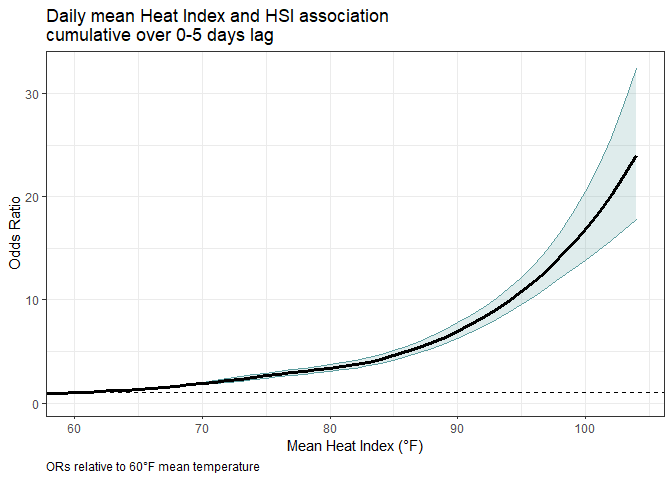
\includegraphics{descriptive_files/figure-latex/unnamed-chunk-4-1.pdf}

\begin{Shaded}
\begin{Highlighting}[]
\NormalTok{cc\_exposure\_df }\SpecialCharTok{\%\textgreater{}\%} 
  \FunctionTok{filter}\NormalTok{(case }\SpecialCharTok{==} \DecValTok{1}\NormalTok{) }\SpecialCharTok{\%\textgreater{}\%} 
  \FunctionTok{group\_by}\NormalTok{(lubridate}\SpecialCharTok{::}\FunctionTok{year}\NormalTok{(date), installation\_name) }\SpecialCharTok{\%\textgreater{}\%} 
  \FunctionTok{count}\NormalTok{() }\SpecialCharTok{\%\textgreater{}\%} 
  \FunctionTok{rename}\NormalTok{(}\AttributeTok{year =} \StringTok{\textasciigrave{}}\AttributeTok{lubridate::year(date)}\StringTok{\textasciigrave{}}\NormalTok{) }\SpecialCharTok{\%\textgreater{}\%} 
  \FunctionTok{ggplot}\NormalTok{(}\FunctionTok{aes}\NormalTok{(}\AttributeTok{x =}\NormalTok{ year, }\AttributeTok{y =}\NormalTok{ n, }\AttributeTok{colour =}\NormalTok{ installation\_name)) }\SpecialCharTok{+}
      \FunctionTok{geom\_point}\NormalTok{() }\SpecialCharTok{+}
      \FunctionTok{geom\_line}\NormalTok{(}\AttributeTok{size =} \FloatTok{0.8}\NormalTok{) }\SpecialCharTok{+}
      \FunctionTok{theme\_bw}\NormalTok{() }\SpecialCharTok{+}
  \FunctionTok{labs}\NormalTok{(}\AttributeTok{title =} \StringTok{"HSI cases by year"}\NormalTok{,}
       \AttributeTok{x =} \StringTok{"year"}\NormalTok{)}
\end{Highlighting}
\end{Shaded}

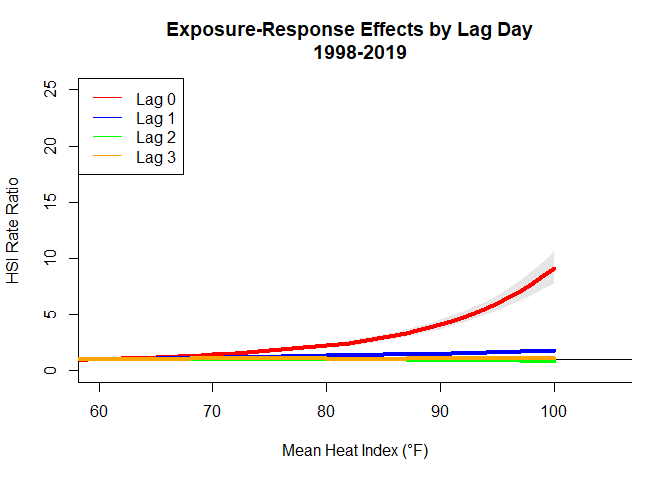
\includegraphics{descriptive_files/figure-latex/unnamed-chunk-4-2.pdf}

\hypertarget{exposures}{%
\subsection{Exposures}\label{exposures}}

\begin{Shaded}
\begin{Highlighting}[]
\CommentTok{\#Density plot, all case days 1998{-}2018, WBGT}


\NormalTok{to\_density\_plot }\OtherTok{\textless{}{-}}
\NormalTok{  cc\_exposure\_df }\SpecialCharTok{\%\textgreater{}\%}
    \FunctionTok{filter}\NormalTok{(case }\SpecialCharTok{==} \DecValTok{1}\NormalTok{) }\SpecialCharTok{\%\textgreater{}\%} 
\NormalTok{    dplyr}\SpecialCharTok{::}\FunctionTok{select}\NormalTok{(installation\_name, d\_event, wbgt\_mean, wbgt\_max) }\SpecialCharTok{\%\textgreater{}\%} 
    \FunctionTok{mutate}\NormalTok{(}\StringTok{"Mean WBGT"} \OtherTok{=}\NormalTok{ weathermetrics}\SpecialCharTok{::}\FunctionTok{celsius.to.fahrenheit}\NormalTok{(wbgt\_mean),}
           \StringTok{"Max WBGT"} \OtherTok{=}\NormalTok{ weathermetrics}\SpecialCharTok{::}\FunctionTok{celsius.to.fahrenheit}\NormalTok{(wbgt\_max)) }\SpecialCharTok{\%\textgreater{}\%} 
\NormalTok{    dplyr}\SpecialCharTok{::}\FunctionTok{select}\NormalTok{(installation\_name, }\StringTok{\textasciigrave{}}\AttributeTok{Mean WBGT}\StringTok{\textasciigrave{}}\NormalTok{, }\StringTok{\textasciigrave{}}\AttributeTok{Max WBGT}\StringTok{\textasciigrave{}}\NormalTok{) }\SpecialCharTok{\%\textgreater{}\%} 
    \FunctionTok{pivot\_longer}\NormalTok{(}\SpecialCharTok{{-}}\NormalTok{installation\_name, }\AttributeTok{names\_to =} \StringTok{"Index"}\NormalTok{, }\AttributeTok{values\_to =} \StringTok{"Value"}\NormalTok{)}

  
\CommentTok{\#check for missing values}
\NormalTok{  to\_density\_plot[}\SpecialCharTok{!}\FunctionTok{complete.cases}\NormalTok{(to\_density\_plot),]}
\end{Highlighting}
\end{Shaded}

\begin{verbatim}
## # A tibble: 0 x 3
## # ... with 3 variables: installation_name <fct>, Index <chr>, Value <dbl>
\end{verbatim}

\begin{Shaded}
\begin{Highlighting}[]
\NormalTok{to\_density\_plot }\SpecialCharTok{\%\textgreater{}\%}   
  \FunctionTok{ggplot}\NormalTok{(}\FunctionTok{aes}\NormalTok{(}\AttributeTok{x =}\NormalTok{ Value, }\AttributeTok{fill =}\NormalTok{ Index, }\AttributeTok{colour =}\NormalTok{ Index)) }\SpecialCharTok{+}
      \FunctionTok{geom\_density}\NormalTok{(}\AttributeTok{alpha =} \FloatTok{0.5}\NormalTok{) }\SpecialCharTok{+}
      \FunctionTok{geom\_rug}\NormalTok{() }\SpecialCharTok{+}
      \FunctionTok{theme\_bw}\NormalTok{() }\SpecialCharTok{+}
  \FunctionTok{labs}\NormalTok{(}\AttributeTok{title =} \StringTok{"Density plot of daily indices on all case days, 1998{-}2019"}\NormalTok{,}
       \AttributeTok{x =} \StringTok{"Daily Index Value (°F)"}\NormalTok{)}
\end{Highlighting}
\end{Shaded}

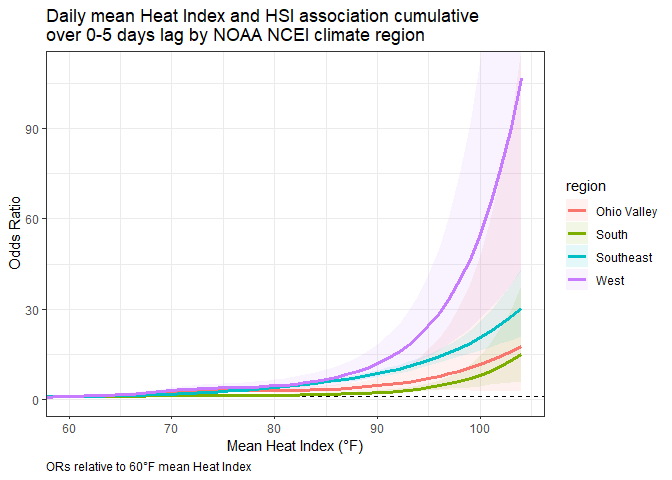
\includegraphics{descriptive_files/figure-latex/unnamed-chunk-5-1.pdf}

\begin{Shaded}
\begin{Highlighting}[]
\NormalTok{to\_density\_plot }\SpecialCharTok{\%\textgreater{}\%} 
  \FunctionTok{group\_by}\NormalTok{(Index) }\SpecialCharTok{\%\textgreater{}\%} 
  \FunctionTok{summarise}\NormalTok{(}\AttributeTok{Mean =} \FunctionTok{mean}\NormalTok{(Value),}
            \AttributeTok{SD =} \FunctionTok{sd}\NormalTok{(Value),}
            \StringTok{\textasciigrave{}}\AttributeTok{75th}\StringTok{\textasciigrave{}} \OtherTok{=} \FunctionTok{quantile}\NormalTok{(Value, .}\DecValTok{75}\NormalTok{),}
            \StringTok{\textasciigrave{}}\AttributeTok{95th}\StringTok{\textasciigrave{}} \OtherTok{=} \FunctionTok{quantile}\NormalTok{(Value, .}\DecValTok{95}\NormalTok{),}
            \AttributeTok{IQR =} \FunctionTok{IQR}\NormalTok{(Value)) }\SpecialCharTok{\%\textgreater{}\%} 
\NormalTok{  knitr}\SpecialCharTok{::}\FunctionTok{kable}\NormalTok{()}
\end{Highlighting}
\end{Shaded}

\begin{verbatim}
## `summarise()` ungrouping output (override with `.groups` argument)
\end{verbatim}

\begin{longtable}[]{@{}lrrrrr@{}}
\toprule
Index & Mean & SD & 75th & 95th & IQR\tabularnewline
\midrule
\endhead
Max WBGT & 80.57825 & 10.25491 & 87.29 & 91.58 & 11.00\tabularnewline
Mean WBGT & 71.83890 & 10.54947 & 79.53 & 82.59 & 12.66\tabularnewline
\bottomrule
\end{longtable}

\begin{Shaded}
\begin{Highlighting}[]
\DocumentationTok{\#\# Day of year}

\NormalTok{cc\_exposure\_df }\SpecialCharTok{\%\textgreater{}\%}
  \FunctionTok{filter}\NormalTok{(case }\SpecialCharTok{==} \DecValTok{1}\NormalTok{) }\SpecialCharTok{\%\textgreater{}\%} 
\NormalTok{  dplyr}\SpecialCharTok{::}\FunctionTok{select}\NormalTok{(installation\_name, date) }\SpecialCharTok{\%\textgreater{}\%} 
  \FunctionTok{mutate}\NormalTok{(}\StringTok{\textasciigrave{}}\AttributeTok{Day of Year}\StringTok{\textasciigrave{}} \OtherTok{=}\NormalTok{ lubridate}\SpecialCharTok{::}\FunctionTok{yday}\NormalTok{(date)) }\SpecialCharTok{\%\textgreater{}\%} 
  \FunctionTok{ggplot}\NormalTok{(}\FunctionTok{aes}\NormalTok{(}\AttributeTok{x =} \StringTok{\textasciigrave{}}\AttributeTok{Day of Year}\StringTok{\textasciigrave{}}\NormalTok{)) }\SpecialCharTok{+}
  \FunctionTok{geom\_density}\NormalTok{(}\AttributeTok{colour =} \StringTok{"cadetblue"}\NormalTok{, }\AttributeTok{fill =} \StringTok{"cadetblue"}\NormalTok{, }\AttributeTok{alpha =} \FloatTok{0.5}\NormalTok{) }\SpecialCharTok{+}
  \FunctionTok{theme\_bw}\NormalTok{() }\SpecialCharTok{+}
  \FunctionTok{labs}\NormalTok{(}\AttributeTok{title =} \StringTok{"Day of year for HSI case days, 1998{-}2019"}\NormalTok{)}
\end{Highlighting}
\end{Shaded}

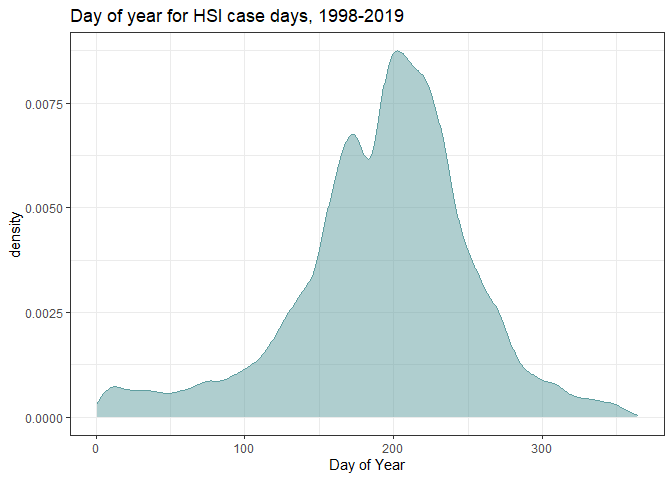
\includegraphics{descriptive_files/figure-latex/unnamed-chunk-5-2.pdf}

\begin{Shaded}
\begin{Highlighting}[]
\NormalTok{cc\_exposure\_df }\SpecialCharTok{\%\textgreater{}\%}
  \FunctionTok{filter}\NormalTok{(case }\SpecialCharTok{==} \DecValTok{1}\NormalTok{) }\SpecialCharTok{\%\textgreater{}\%} 
\NormalTok{  dplyr}\SpecialCharTok{::}\FunctionTok{select}\NormalTok{(installation\_name, date) }\SpecialCharTok{\%\textgreater{}\%} 
  \FunctionTok{mutate}\NormalTok{(}\StringTok{\textasciigrave{}}\AttributeTok{Day of Year}\StringTok{\textasciigrave{}} \OtherTok{=}\NormalTok{ lubridate}\SpecialCharTok{::}\FunctionTok{yday}\NormalTok{(date)) }\SpecialCharTok{\%\textgreater{}\%} 
  \FunctionTok{ggplot}\NormalTok{(}\FunctionTok{aes}\NormalTok{(}\AttributeTok{x =} \StringTok{\textasciigrave{}}\AttributeTok{Day of Year}\StringTok{\textasciigrave{}}\NormalTok{)) }\SpecialCharTok{+}
  \FunctionTok{geom\_bar}\NormalTok{(}\AttributeTok{colour =} \StringTok{"cadetblue"}\NormalTok{, }\AttributeTok{fill =} \StringTok{"cadetblue"}\NormalTok{, }\AttributeTok{alpha =} \FloatTok{0.5}\NormalTok{) }\SpecialCharTok{+}
  \FunctionTok{theme\_bw}\NormalTok{() }\SpecialCharTok{+}
  \FunctionTok{labs}\NormalTok{(}\AttributeTok{title =} \StringTok{"Day of year for HSI case days, 1998{-}2019"}\NormalTok{)}
\end{Highlighting}
\end{Shaded}

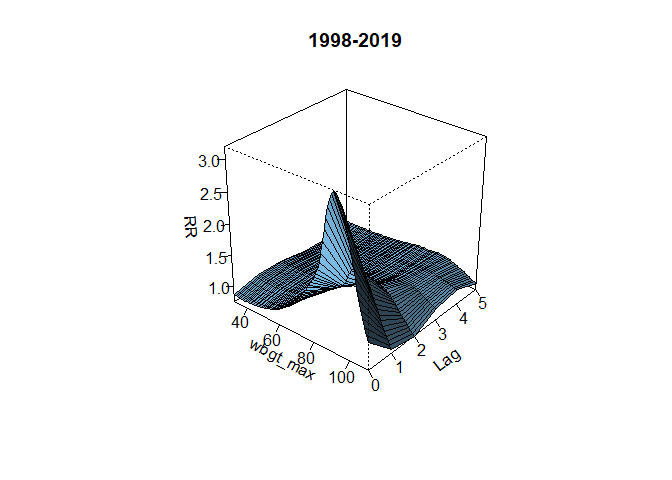
\includegraphics{descriptive_files/figure-latex/unnamed-chunk-5-3.pdf}

\hypertarget{temperature-indices}{%
\subsection{Temperature indices}\label{temperature-indices}}

\begin{Shaded}
\begin{Highlighting}[]
\CommentTok{\#Density plot, all case days 1998{-}2018, Temp}


\NormalTok{to\_density\_plot }\OtherTok{\textless{}{-}}
\NormalTok{  cc\_exposure\_df }\SpecialCharTok{\%\textgreater{}\%}
    \FunctionTok{filter}\NormalTok{(case }\SpecialCharTok{==} \DecValTok{1}\NormalTok{) }\SpecialCharTok{\%\textgreater{}\%} 
\NormalTok{    dplyr}\SpecialCharTok{::}\FunctionTok{select}\NormalTok{(installation\_name, d\_event, tmp\_f\_mean, tmp\_f\_max) }\SpecialCharTok{\%\textgreater{}\%} 
    \FunctionTok{rename}\NormalTok{(}\StringTok{"Mean Temp"} \OtherTok{=}\NormalTok{ tmp\_f\_mean,}
           \StringTok{"Max Temp"} \OtherTok{=}\NormalTok{ tmp\_f\_max) }\SpecialCharTok{\%\textgreater{}\%} 
\NormalTok{    dplyr}\SpecialCharTok{::}\FunctionTok{select}\NormalTok{(installation\_name, }\StringTok{\textasciigrave{}}\AttributeTok{Mean Temp}\StringTok{\textasciigrave{}}\NormalTok{, }\StringTok{\textasciigrave{}}\AttributeTok{Max Temp}\StringTok{\textasciigrave{}}\NormalTok{) }\SpecialCharTok{\%\textgreater{}\%} 
    \FunctionTok{pivot\_longer}\NormalTok{(}\SpecialCharTok{{-}}\NormalTok{installation\_name, }\AttributeTok{names\_to =} \StringTok{"Index"}\NormalTok{, }\AttributeTok{values\_to =} \StringTok{"Value"}\NormalTok{)}

  
\CommentTok{\#check for missing values}
\NormalTok{  to\_density\_plot[}\SpecialCharTok{!}\FunctionTok{complete.cases}\NormalTok{(to\_density\_plot),] }
\end{Highlighting}
\end{Shaded}

\begin{verbatim}
## # A tibble: 0 x 3
## # ... with 3 variables: installation_name <fct>, Index <chr>, Value <dbl>
\end{verbatim}

\begin{Shaded}
\begin{Highlighting}[]
\NormalTok{to\_density\_plot }\SpecialCharTok{\%\textgreater{}\%}   
  \FunctionTok{ggplot}\NormalTok{(}\FunctionTok{aes}\NormalTok{(}\AttributeTok{x =}\NormalTok{ Value, }\AttributeTok{fill =}\NormalTok{ Index, }\AttributeTok{colour =}\NormalTok{ Index)) }\SpecialCharTok{+}
      \FunctionTok{geom\_density}\NormalTok{(}\AttributeTok{alpha =} \FloatTok{0.5}\NormalTok{) }\SpecialCharTok{+}
      \FunctionTok{geom\_rug}\NormalTok{() }\SpecialCharTok{+}
      \FunctionTok{theme\_bw}\NormalTok{() }\SpecialCharTok{+}
  \FunctionTok{labs}\NormalTok{(}\AttributeTok{title =} \StringTok{"Density plot of daily indices on all case days, 1998{-}2019"}\NormalTok{,}
       \AttributeTok{x =} \StringTok{"Daily Index Value (°F)"}\NormalTok{)}
\end{Highlighting}
\end{Shaded}

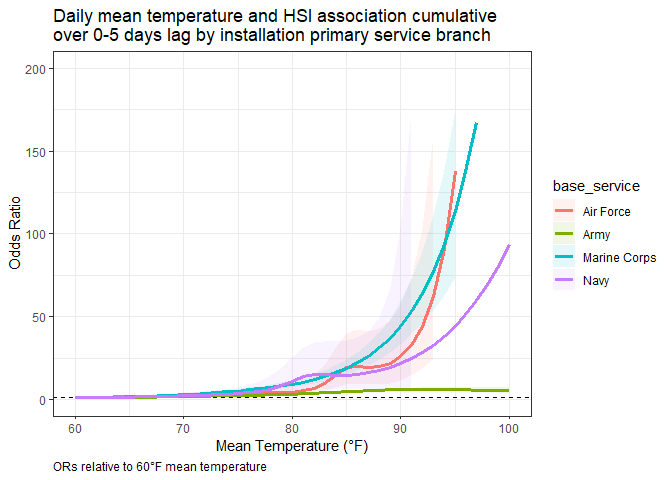
\includegraphics{descriptive_files/figure-latex/unnamed-chunk-6-1.pdf}

\begin{Shaded}
\begin{Highlighting}[]
\NormalTok{to\_density\_plot }\SpecialCharTok{\%\textgreater{}\%} 
  \FunctionTok{group\_by}\NormalTok{(Index) }\SpecialCharTok{\%\textgreater{}\%} 
  \FunctionTok{summarise}\NormalTok{(}\AttributeTok{Mean =} \FunctionTok{mean}\NormalTok{(Value),}
            \AttributeTok{SD =} \FunctionTok{sd}\NormalTok{(Value),}
            \StringTok{\textasciigrave{}}\AttributeTok{75th}\StringTok{\textasciigrave{}} \OtherTok{=} \FunctionTok{quantile}\NormalTok{(Value, .}\DecValTok{75}\NormalTok{),}
            \StringTok{\textasciigrave{}}\AttributeTok{95th}\StringTok{\textasciigrave{}} \OtherTok{=} \FunctionTok{quantile}\NormalTok{(Value, .}\DecValTok{95}\NormalTok{),}
            \AttributeTok{IQR =} \FunctionTok{IQR}\NormalTok{(Value)) }\SpecialCharTok{\%\textgreater{}\%} 
\NormalTok{  knitr}\SpecialCharTok{::}\FunctionTok{kable}\NormalTok{()}
\end{Highlighting}
\end{Shaded}

\begin{verbatim}
## `summarise()` ungrouping output (override with `.groups` argument)
\end{verbatim}

\begin{longtable}[]{@{}lrrrrr@{}}
\toprule
Index & Mean & SD & 75th & 95th & IQR\tabularnewline
\midrule
\endhead
Max Temp & 85.38130 & 12.28294 & 92.86000 & 101.66000 &
11.95000\tabularnewline
Mean Temp & 76.54029 & 11.45315 & 83.92958 & 89.44777 &
12.45052\tabularnewline
\bottomrule
\end{longtable}

\hypertarget{map}{%
\subsection{Map}\label{map}}

\begin{Shaded}
\begin{Highlighting}[]
\NormalTok{centroid\_coords }\OtherTok{\textless{}{-}}
  \FunctionTok{read\_rds}\NormalTok{(}\StringTok{"data/centroid\_coords.rds"}\NormalTok{)}



\NormalTok{centroid\_coords}\SpecialCharTok{$}\NormalTok{site\_name }
\end{Highlighting}
\end{Shaded}

\begin{verbatim}
##  [1] "Fort Benning GA"                 "Fort Campbell"                  
##  [3] "NAS Pensacola"                   "Naval Medical Center Portsmouth"
##  [5] "MCB Quantico"                    "MCRD San Diego"                 
##  [7] "Fort Huachuca"                   "Fort Riley"                     
##  [9] "NTC and Fort Irwin"              "Fort Gordon"                    
## [11] "Twentynine Palms Main Base"      "Fort Sill"                      
## [13] "Fort Carson"                     "Fort Lewis"                     
## [15] "MCB Camp Lejeune"                "MCRD Beaufort Parris Island"    
## [17] "MCB Camp Pendleton"              "Fort Bragg"                     
## [19] "Eglin AFB"                       "Lackland AFB"                   
## [21] "Fort Sam Houston"                "West Point Mil Reservation"     
## [23] "Fort Polk"                       "Fort Jackson"                   
## [25] "Fort Leonard Wood"               "Fort Bliss"                     
## [27] "Fort Hood"                       "Fort Drum"                      
## [29] "Fort Stewart"                    "Fort Knox"
\end{verbatim}

\begin{Shaded}
\begin{Highlighting}[]
\NormalTok{centroid\_coords}\SpecialCharTok{$}\NormalTok{geometry }
\end{Highlighting}
\end{Shaded}

\begin{verbatim}
## Geometry set for 30 features 
## geometry type:  MULTIPOLYGON
## dimension:      XY
## bbox:           xmin: -123.9623 ymin: 29.36673 xmax: -73.95086 ymax: 47.21875
## geographic CRS: WGS 84
## First 5 geometries:
\end{verbatim}

\begin{verbatim}
## MULTIPOLYGON (((-84.75323 32.54967, -84.7524 32...
\end{verbatim}

\begin{verbatim}
## MULTIPOLYGON (((-87.65135 36.54532, -87.65779 3...
\end{verbatim}

\begin{verbatim}
## MULTIPOLYGON (((-87.32506 30.33455, -87.32506 3...
\end{verbatim}

\begin{verbatim}
## MULTIPOLYGON (((-76.31359 36.84893, -76.3135 36...
\end{verbatim}

\begin{verbatim}
## MULTIPOLYGON (((-77.4884 38.63829, -77.48829 38...
\end{verbatim}

\begin{Shaded}
\begin{Highlighting}[]
\CommentTok{\# convert Installation names from snake{-}case to "title"}
\NormalTok{base\_service\_df }\OtherTok{\textless{}{-}}
\NormalTok{  base\_service\_df }\SpecialCharTok{\%\textgreater{}\%}
    \FunctionTok{mutate}\NormalTok{(}\AttributeTok{installation\_name =} \FunctionTok{str\_replace\_all}\NormalTok{(installation\_name, }\StringTok{"\_"}\NormalTok{, }\StringTok{" "}\NormalTok{),}
      \AttributeTok{installation\_name =} \FunctionTok{str\_to\_title}\NormalTok{(installation\_name, }\AttributeTok{locale =} \StringTok{"en"}\NormalTok{))}

\NormalTok{base\_service\_df}\SpecialCharTok{$}\NormalTok{installation\_name}
\end{Highlighting}
\end{Shaded}

\begin{verbatim}
##  [1] "Fort Benning"       "Fort Bragg"         "Camp Lejeune"      
##  [4] "Parris Island"      "Fort Campbell"      "Fort Polk"         
##  [7] "Fort Jackson"       "Camp Pendleton"     "Fort Hood"         
## [10] "Mcrd San Diego"     "Fort Stewart"       "Jbsa"              
## [13] "Quantico"           "Twentynine Palms"   "Fort Sill"         
## [16] "Fort Leonard Wood"  "Fort Riley"         "Ntc And Fort Irwin"
## [19] "Fort Knox"          "Fort Bliss"         "Portsmouth"        
## [22] "Pensacola"          "Fort Gordon"        "Eglin Afb"
\end{verbatim}

\begin{Shaded}
\begin{Highlighting}[]
\CommentTok{\# Change \textasciigrave{}centroid\_coords\textasciigrave{} site names to match}

\NormalTok{centroid\_coords }\OtherTok{\textless{}{-}}
\NormalTok{  centroid\_coords }\SpecialCharTok{\%\textgreater{}\%} 
    \FunctionTok{mutate}\NormalTok{(}\AttributeTok{site\_name =} \FunctionTok{recode}\NormalTok{(site\_name,}
                              \StringTok{"Fort Benning GA"} \OtherTok{=} \StringTok{"Fort Benning"}\NormalTok{,}
                              \StringTok{"NAS Pensacola"} \OtherTok{=} \StringTok{"Pensacola"}\NormalTok{,}
                              \StringTok{"Naval Medical Center Portsmouth"} \OtherTok{=} \StringTok{"Portsmouth"}\NormalTok{,}
                              \StringTok{"MCB Quantico"} \OtherTok{=} \StringTok{"Quantico"}\NormalTok{,}
                              \StringTok{"MCRD San Diego"} \OtherTok{=} \StringTok{"Mcrd San Diego"}\NormalTok{,}
                              \StringTok{"NTC and Fort Irwin"} \OtherTok{=} \StringTok{"Ntc And Fort Irwin"}\NormalTok{,}
                              \StringTok{"Twentynine Palms Main Base"} \OtherTok{=} \StringTok{"Twentynine Palms"}\NormalTok{,}
                              \StringTok{"MCB Camp Lejeune"} \OtherTok{=} \StringTok{"Camp Lejeune"}\NormalTok{,}
                              \StringTok{"Eglin AFB"} \OtherTok{=} \StringTok{"Eglin Afb"}\NormalTok{,}
                              \StringTok{"Fort Sam Houston"} \OtherTok{=} \StringTok{"Jbsa"}\NormalTok{,}
                              \StringTok{"MCRD Beaufort Parris Island"} \OtherTok{=} \StringTok{"Parris Island"}\NormalTok{,}
                              \StringTok{"MCB Camp Pendleton"} \OtherTok{=} \StringTok{"Camp Pendleton"}\NormalTok{))}


\NormalTok{mapping\_df }\OtherTok{\textless{}{-}}
\NormalTok{  base\_service\_df }\SpecialCharTok{\%\textgreater{}\%} 
    \FunctionTok{left\_join}\NormalTok{(centroid\_coords, }\AttributeTok{by =} \FunctionTok{c}\NormalTok{(}\StringTok{"installation\_name"} \OtherTok{=} \StringTok{"site\_name"}\NormalTok{))}

\CommentTok{\#write\_rds(mapping\_df, file = "data/mapping\_df.rds")}
                              


\NormalTok{mapping\_df                              }
\end{Highlighting}
\end{Shaded}

\begin{verbatim}
## # A tibble: 24 x 11
##    installation_na~     A     C     F     M     N service region state_terr
##    <chr>            <dbl> <dbl> <dbl> <dbl> <dbl> <chr>   <chr>  <chr>     
##  1 Fort Benning     20600     0    44    98    53 Army    South~ Georgia   
##  2 Fort Bragg       20546     0   376    23    19 Army    South~ North Car~
##  3 Camp Lejeune        48    29    12 11721  1387 Marine~ South~ North Car~
##  4 Parris Island        4     0     0 10804    68 Marine~ South~ South Car~
##  5 Fort Campbell     8738     5    21     0     9 Army    Ohio ~ Kentucky  
##  6 Fort Polk         7396     0    53    12     5 Army    South  Louisiana 
##  7 Fort Jackson      7495     0   151    13   123 Army    South~ South Car~
##  8 Camp Pendleton      36     5     4  6137   413 Marine~ West   California
##  9 Fort Hood         5412     4    21   184   209 Army    South  Texas     
## 10 Mcrd San Diego      38    18     5  4031  1035 Marine~ West   California
## # ... with 14 more rows, and 2 more variables: geometry <MULTIPOLYGON [°]>,
## #   centroid <POINT [°]>
\end{verbatim}

\begin{Shaded}
\begin{Highlighting}[]
\NormalTok{point\_coords }\OtherTok{\textless{}{-}}
  \FunctionTok{st\_coordinates}\NormalTok{(mapping\_df}\SpecialCharTok{$}\NormalTok{centroid) }\SpecialCharTok{\%\textgreater{}\%} 
    \FunctionTok{as\_tibble}\NormalTok{() }\SpecialCharTok{\%\textgreater{}\%} 
    \FunctionTok{rename}\NormalTok{(}\StringTok{"longitude"} \OtherTok{=} \StringTok{"X"}\NormalTok{,}
           \StringTok{"latitude"} \OtherTok{=} \StringTok{"Y"}\NormalTok{)}


\NormalTok{mapping\_df }\OtherTok{\textless{}{-}}
\NormalTok{  mapping\_df }\SpecialCharTok{\%\textgreater{}\%} \FunctionTok{bind\_cols}\NormalTok{(}
\NormalTok{    point\_coords)}



\NormalTok{sites }\OtherTok{\textless{}{-}} \FunctionTok{data.frame}\NormalTok{(}\AttributeTok{names =}\NormalTok{ mapping\_df}\SpecialCharTok{$}\NormalTok{installation\_name,}
                    \AttributeTok{longitude =}\NormalTok{ mapping\_df}\SpecialCharTok{$}\NormalTok{longitude,}
                    \AttributeTok{latitude =}\NormalTok{ mapping\_df}\SpecialCharTok{$}\NormalTok{latitude,}
                    \AttributeTok{region =}\NormalTok{ mapping\_df}\SpecialCharTok{$}\NormalTok{region,}
                    \AttributeTok{service =}\NormalTok{ mapping\_df}\SpecialCharTok{$}\NormalTok{service)}


\NormalTok{sites }\OtherTok{\textless{}{-}} \FunctionTok{st\_as\_sf}\NormalTok{(sites, }\AttributeTok{coords =} \FunctionTok{c}\NormalTok{(}\StringTok{"longitude"}\NormalTok{, }\StringTok{"latitude"}\NormalTok{), }\AttributeTok{remove =} \ConstantTok{FALSE}\NormalTok{, }
    \AttributeTok{crs =} \DecValTok{4326}\NormalTok{, }\AttributeTok{agr =} \StringTok{"constant"}\NormalTok{)}



\CommentTok{\#world map}

\NormalTok{world }\OtherTok{\textless{}{-}} \FunctionTok{ne\_countries}\NormalTok{(}\AttributeTok{scale =} \StringTok{"medium"}\NormalTok{, }\AttributeTok{returnclass =} \StringTok{"sf"}\NormalTok{)}
\NormalTok{usa }\OtherTok{\textless{}{-}} \FunctionTok{ne\_countries}\NormalTok{(}\AttributeTok{country =} \StringTok{\textquotesingle{}united states of america\textquotesingle{}}\NormalTok{, }\AttributeTok{scale =} \StringTok{"medium"}\NormalTok{, }\AttributeTok{returnclass =} \StringTok{"sf"}\NormalTok{)}
\NormalTok{usa}
\end{Highlighting}
\end{Shaded}

\begin{verbatim}
## Simple feature collection with 1 feature and 63 fields
## geometry type:  MULTIPOLYGON
## dimension:      XY
## bbox:           xmin: -178.1945 ymin: 18.96392 xmax: 179.78 ymax: 71.40767
## CRS:            +proj=longlat +datum=WGS84 +no_defs +ellps=WGS84 +towgs84=0,0,0
##     scalerank      featurecla labelrank               sovereignt sov_a3
## 226         1 Admin-0 country         2 United States of America    US1
##     adm0_dif level    type                    admin adm0_a3 geou_dif
## 226        1     2 Country United States of America     USA        0
##                      geounit gu_a3 su_dif                  subunit su_a3
## 226 United States of America   USA      0 United States of America   USA
##     brk_diff          name     name_long brk_a3      brk_name brk_group abbrev
## 226        0 United States United States    USA United States      <NA> U.S.A.
##     postal                formal_en formal_fr note_adm0 note_brk
## 226     US United States of America      <NA>      <NA>     <NA>
##                    name_sort name_alt mapcolor7 mapcolor8 mapcolor9 mapcolor13
## 226 United States of America     <NA>         4         5         1          1
##       pop_est gdp_md_est pop_year lastcensus gdp_year                 economy
## 226 313973000   15094000        0       2010        0 1. Developed region: G7
##               income_grp wikipedia fips_10 iso_a2 iso_a3 iso_n3 un_a3 wb_a2
## 226 1. High income: OECD         0    <NA>     US    USA    840   840    US
##     wb_a3 woe_id adm0_a3_is adm0_a3_us adm0_a3_un adm0_a3_wb     continent
## 226   USA     NA        USA        USA         NA         NA North America
##     region_un        subregion     region_wb name_len long_len abbrev_len tiny
## 226  Americas Northern America North America       13       13          6   NA
##     homepart                       geometry
## 226        1 MULTIPOLYGON (((-155.5813 1...
\end{verbatim}

\begin{Shaded}
\begin{Highlighting}[]
\NormalTok{states }\OtherTok{\textless{}{-}} \FunctionTok{st\_as\_sf}\NormalTok{(}\FunctionTok{map}\NormalTok{(}\StringTok{"state"}\NormalTok{, }\AttributeTok{plot =} \ConstantTok{FALSE}\NormalTok{, }\AttributeTok{fill =} \ConstantTok{TRUE}\NormalTok{))}
\NormalTok{states}
\end{Highlighting}
\end{Shaded}

\begin{verbatim}
## Simple feature collection with 49 features and 1 field
## geometry type:  MULTIPOLYGON
## dimension:      XY
## bbox:           xmin: -124.6813 ymin: 25.12993 xmax: -67.00742 ymax: 49.38323
## geographic CRS: WGS 84
## First 10 features:
##                      ID                           geom
## 1               alabama MULTIPOLYGON (((-87.46201 3...
## 2               arizona MULTIPOLYGON (((-114.6374 3...
## 3              arkansas MULTIPOLYGON (((-94.05103 3...
## 4            california MULTIPOLYGON (((-120.006 42...
## 5              colorado MULTIPOLYGON (((-102.0552 4...
## 6           connecticut MULTIPOLYGON (((-73.49902 4...
## 7              delaware MULTIPOLYGON (((-75.80231 3...
## 8  district of columbia MULTIPOLYGON (((-77.13731 3...
## 9               florida MULTIPOLYGON (((-85.01548 3...
## 10              georgia MULTIPOLYGON (((-80.89018 3...
\end{verbatim}

\begin{Shaded}
\begin{Highlighting}[]
\FunctionTok{ggplot}\NormalTok{(}\AttributeTok{data =}\NormalTok{ usa) }\SpecialCharTok{+}
    \FunctionTok{geom\_sf}\NormalTok{() }\SpecialCharTok{+}
    \FunctionTok{geom\_sf}\NormalTok{(}\AttributeTok{data =}\NormalTok{ states, }\AttributeTok{fill =} \StringTok{"cornsilk"}\NormalTok{) }\SpecialCharTok{+} 
    \FunctionTok{geom\_point}\NormalTok{(}\AttributeTok{data =}\NormalTok{ sites, }\FunctionTok{aes}\NormalTok{(}\AttributeTok{x =}\NormalTok{ longitude, }\AttributeTok{y =}\NormalTok{ latitude, }\AttributeTok{fill =}\NormalTok{ service), }\AttributeTok{size =} \DecValTok{4}\NormalTok{, }
        \AttributeTok{shape =} \DecValTok{23}\NormalTok{) }\SpecialCharTok{+}
    \FunctionTok{geom\_sf}\NormalTok{(}\AttributeTok{data =}\NormalTok{ sites) }\SpecialCharTok{+}
    \FunctionTok{geom\_text\_repel}\NormalTok{(}\AttributeTok{data =}\NormalTok{ sites, }\FunctionTok{aes}\NormalTok{(}\AttributeTok{x =}\NormalTok{ longitude, }\AttributeTok{y =}\NormalTok{ latitude, }\AttributeTok{label =}\NormalTok{ names), }\AttributeTok{fontface =} \StringTok{"bold"}\NormalTok{, }\AttributeTok{size =} \DecValTok{3}\NormalTok{, }
        \AttributeTok{nudge\_x =} \DecValTok{3}\NormalTok{, }\AttributeTok{nudge\_y =} \SpecialCharTok{{-}}\DecValTok{2}\NormalTok{) }\SpecialCharTok{+}
    \FunctionTok{coord\_sf}\NormalTok{(}\AttributeTok{xlim =} \FunctionTok{c}\NormalTok{(}\SpecialCharTok{{-}}\DecValTok{130}\NormalTok{, }\SpecialCharTok{{-}}\DecValTok{65}\NormalTok{), }\AttributeTok{ylim =} \FunctionTok{c}\NormalTok{(}\FloatTok{24.5}\NormalTok{, }\DecValTok{50}\NormalTok{), }\AttributeTok{expand =} \ConstantTok{FALSE}\NormalTok{) }\SpecialCharTok{+}
    \FunctionTok{ggtitle}\NormalTok{(}\StringTok{"Study Installations"}\NormalTok{, }\AttributeTok{subtitle =} \StringTok{"(n=24)"}\NormalTok{) }\SpecialCharTok{+}
    \FunctionTok{theme}\NormalTok{(}\AttributeTok{panel.grid.major =} \FunctionTok{element\_line}\NormalTok{(}\AttributeTok{color =} \FunctionTok{gray}\NormalTok{(}\FloatTok{0.5}\NormalTok{), }\AttributeTok{linetype =} \StringTok{"dashed"}\NormalTok{, }
        \AttributeTok{size =} \FloatTok{0.5}\NormalTok{), }\AttributeTok{panel.background =} \FunctionTok{element\_rect}\NormalTok{(}\AttributeTok{fill =} \StringTok{"azure2"}\NormalTok{))}
\end{Highlighting}
\end{Shaded}

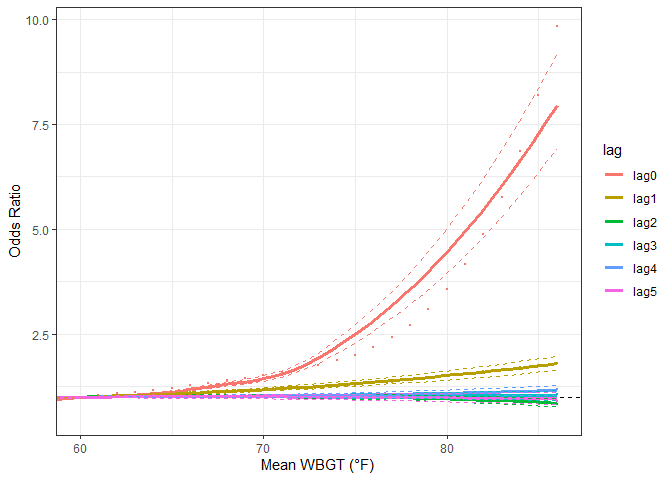
\includegraphics{descriptive_files/figure-latex/unnamed-chunk-8-1.pdf}

\begin{Shaded}
\begin{Highlighting}[]
\CommentTok{\# ggsave("output/study\_map.png")}
\end{Highlighting}
\end{Shaded}

\hypertarget{earlier-descriptive-review}{%
\subsection{Earlier descriptive
review}\label{earlier-descriptive-review}}

Read in daily NLDAS

\begin{Shaded}
\begin{Highlighting}[]
\NormalTok{daily\_nldas }\OtherTok{\textless{}{-}} \FunctionTok{read\_rds}\NormalTok{(}\AttributeTok{file =} \StringTok{"E:/data/daily\_nldas.rds"}\NormalTok{)}
\end{Highlighting}
\end{Shaded}

``Table 1''

\begin{Shaded}
\begin{Highlighting}[]
\CommentTok{\# Outcomes }

\NormalTok{cc\_exposure\_df }\OtherTok{\textless{}{-}}
  \FunctionTok{read\_rds}\NormalTok{(}\AttributeTok{file =} \StringTok{"E:/data/cc\_exposure\_df.rds"}\NormalTok{)}

\NormalTok{table1}\SpecialCharTok{::}\FunctionTok{table1}\NormalTok{(}\SpecialCharTok{\textasciitilde{}} \FunctionTok{factor}\NormalTok{(source) }\SpecialCharTok{+} \FunctionTok{factor}\NormalTok{(hsi) }\SpecialCharTok{+} \FunctionTok{factor}\NormalTok{(service) }\SpecialCharTok{|}\NormalTok{ case, }\AttributeTok{data =}\NormalTok{ cc\_exposure\_df)}


\NormalTok{table1}\SpecialCharTok{::}\FunctionTok{table1}\NormalTok{(}\SpecialCharTok{\textasciitilde{}} \FunctionTok{factor}\NormalTok{(installation\_name) }\SpecialCharTok{|}\NormalTok{ case, }\AttributeTok{data =}\NormalTok{ cc\_exposure\_df)}


\CommentTok{\# Exposure}

\NormalTok{nldas\_1998 }\OtherTok{\textless{}{-}}\NormalTok{ daily\_nldas }\SpecialCharTok{\%\textgreater{}\%} 
  \FunctionTok{filter}\NormalTok{(lubridate}\SpecialCharTok{::}\FunctionTok{year}\NormalTok{(date) }\SpecialCharTok{\%in\%} \DecValTok{1998}\SpecialCharTok{:}\DecValTok{2019}\NormalTok{)}

\NormalTok{table1}\SpecialCharTok{::}\FunctionTok{table1}\NormalTok{(}\SpecialCharTok{\textasciitilde{}}\NormalTok{ tmp\_f\_mean }\SpecialCharTok{+}\NormalTok{ heat\_index\_mean }\SpecialCharTok{+}\NormalTok{ Twbg\_u\_mean }\SpecialCharTok{|} \FunctionTok{factor}\NormalTok{(installation), }\AttributeTok{data =}\NormalTok{ nldas\_1998)}

\CommentTok{\# Indiv risk factors}

\NormalTok{table1}\SpecialCharTok{::}\FunctionTok{table1}\NormalTok{(}\SpecialCharTok{\textasciitilde{}} \FunctionTok{factor}\NormalTok{(sex) }\SpecialCharTok{+} \FunctionTok{factor}\NormalTok{(age) }\SpecialCharTok{+} \FunctionTok{factor}\NormalTok{(grade) }\SpecialCharTok{+}\NormalTok{ bmi }\SpecialCharTok{|}\NormalTok{ case, }\AttributeTok{data =}\NormalTok{ cc\_exposure\_df)}
\end{Highlighting}
\end{Shaded}

Compare WBGT to Temp and Heat Index

\begin{Shaded}
\begin{Highlighting}[]
\NormalTok{daily\_nldas }\SpecialCharTok{\%\textgreater{}\%} 
\NormalTok{  drop\_na }\SpecialCharTok{\%\textgreater{}\%} 
  \FunctionTok{filter}\NormalTok{(lubridate}\SpecialCharTok{::}\FunctionTok{year}\NormalTok{(date) }\SpecialCharTok{\%in\%} \DecValTok{1998}\SpecialCharTok{:}\DecValTok{2019}\NormalTok{) }\SpecialCharTok{\%\textgreater{}\%} 
\NormalTok{  dplyr}\SpecialCharTok{::}\FunctionTok{select}\NormalTok{(tmp\_f\_mean, heat\_index\_mean, Twbg\_u\_mean, Tnwb\_u\_mean) }\SpecialCharTok{\%\textgreater{}\%} 
  \FunctionTok{ggplot}\NormalTok{(}\FunctionTok{aes}\NormalTok{(}\AttributeTok{x =}\NormalTok{ tmp\_f\_mean, }\AttributeTok{y =}\NormalTok{ Twbg\_u\_mean, }\AttributeTok{color =}\NormalTok{ installation)) }\SpecialCharTok{+}
    \FunctionTok{geom\_point}\NormalTok{(}\FunctionTok{aes}\NormalTok{(}\AttributeTok{alpha =} \FloatTok{0.2}\NormalTok{, }\AttributeTok{size =} \FloatTok{0.2}\NormalTok{)) }\SpecialCharTok{+}
    \FunctionTok{geom\_smooth}\NormalTok{(}\AttributeTok{method =} \StringTok{"lm"}\NormalTok{) }\SpecialCharTok{+}
    \FunctionTok{theme\_bw}\NormalTok{()}



\NormalTok{daily\_nldas }\SpecialCharTok{\%\textgreater{}\%} 
  \FunctionTok{ungroup}\NormalTok{() }\SpecialCharTok{\%\textgreater{}\%} 
  \FunctionTok{filter}\NormalTok{(lubridate}\SpecialCharTok{::}\FunctionTok{year}\NormalTok{(date) }\SpecialCharTok{\%in\%} \DecValTok{1998}\SpecialCharTok{:}\DecValTok{2019}\NormalTok{) }\SpecialCharTok{\%\textgreater{}\%} 
\NormalTok{  dplyr}\SpecialCharTok{::}\FunctionTok{select}\NormalTok{(tmp\_f\_mean, heat\_index\_mean, Twbg\_u\_mean, Tnwb\_u\_mean) }\SpecialCharTok{\%\textgreater{}\%} 
  \FunctionTok{cor}\NormalTok{()}


\NormalTok{daily\_nldas }\SpecialCharTok{\%\textgreater{}\%} 
  \FunctionTok{filter}\NormalTok{(lubridate}\SpecialCharTok{::}\FunctionTok{year}\NormalTok{(date) }\SpecialCharTok{\%in\%} \DecValTok{1998}\SpecialCharTok{:}\DecValTok{2019}\NormalTok{) }\SpecialCharTok{\%\textgreater{}\%} 
\NormalTok{  dplyr}\SpecialCharTok{::}\FunctionTok{select}\NormalTok{(installation, tmp\_f\_mean, heat\_index\_mean, Twbg\_u\_mean, Tnwb\_u\_mean) }\SpecialCharTok{\%\textgreater{}\%} 
  \FunctionTok{group\_by}\NormalTok{(installation) }\SpecialCharTok{\%\textgreater{}\%} 
    \FunctionTok{summarise}\NormalTok{(}\AttributeTok{r =} \FunctionTok{cor}\NormalTok{(tmp\_f\_mean, Twbg\_u\_mean)) }\SpecialCharTok{\%\textgreater{}\%} \FunctionTok{View}\NormalTok{()}
\end{Highlighting}
\end{Shaded}


\end{document}
